\documentclass[a4paper]{book}
\usepackage{a4wide}
\usepackage{makeidx}
\usepackage{fancyhdr}
\usepackage{graphicx}
\usepackage{multicol}
\usepackage{float}
\usepackage{textcomp}
\usepackage{alltt}
\usepackage{times}
\usepackage{ifpdf}
\ifpdf
\usepackage[pdftex,
            pagebackref=true,
            colorlinks=true,
            linkcolor=blue,
            unicode
           ]{hyperref}
\else
\usepackage[ps2pdf,
            pagebackref=true,
            colorlinks=true,
            linkcolor=blue,
            unicode
           ]{hyperref}
\usepackage{pspicture}
\fi
\usepackage[utf8]{inputenc}
\usepackage[french]{babel}

\usepackage{doxygen}
\makeindex
\setcounter{tocdepth}{3}
\renewcommand{\footrulewidth}{0.4pt}
\begin{document}
\begin{titlepage}
\vspace*{7cm}
\begin{center}
{\Large LO21 - Calculatrice \\[1ex]\large 1 }\\
\vspace*{1cm}
{\large Généré par Doxygen 1.5.8}\\
\vspace*{0.5cm}
{\small Tue Jun 7 19:27:55 2016}\\
\end{center}
\end{titlepage}
\clearemptydoublepage
\pagenumbering{roman}
\tableofcontents
\clearemptydoublepage
\pagenumbering{arabic}
\chapter{Index des classes}
\section{Hiérarchie des classes}
Cette liste d'héritage est classée approximativement par ordre alphabétique :\begin{CompactList}
\item \contentsline{section}{ComputerException}{\pageref{class_computer_exception}}{}
\item \contentsline{section}{Controleur}{\pageref{class_controleur}}{}
\item \contentsline{section}{HashEntry}{\pageref{class_hash_entry}}{}
\item \contentsline{section}{HashMap}{\pageref{class_hash_map}}{}
\item \contentsline{section}{Item}{\pageref{class_item}}{}
\item \contentsline{section}{Litterale}{\pageref{class_litterale}}{}
\begin{CompactList}
\item \contentsline{section}{Atome}{\pageref{class_atome}}{}
\item \contentsline{section}{Complexe}{\pageref{class_complexe}}{}
\item \contentsline{section}{Expression}{\pageref{class_expression}}{}
\item \contentsline{section}{Numerique}{\pageref{class_numerique}}{}
\begin{CompactList}
\item \contentsline{section}{Entiere}{\pageref{class_entiere}}{}
\item \contentsline{section}{Rationnelle}{\pageref{class_rationnelle}}{}
\item \contentsline{section}{Reelle}{\pageref{class_reelle}}{}
\end{CompactList}
\item \contentsline{section}{Programme}{\pageref{class_programme}}{}
\end{CompactList}
\item \contentsline{section}{LitteraleManager}{\pageref{class_litterale_manager}}{}
\item \contentsline{section}{Pile}{\pageref{class_pile}}{}
\end{CompactList}

\chapter{Index des classes}
\section{Liste des classes}
Liste des classes, structures, unions et interfaces avec une brève description :\begin{CompactList}
\item\contentsline{section}{\hyperlink{class_atome}{Atome} (Classe representant un atome, c'est a dire un identificateur (heritage de \hyperlink{class_litterale}{Litterale}) )}{\pageref{class_atome}}{}
\item\contentsline{section}{\hyperlink{class_complexe}{Complexe} (Classe representant un nombre complexe (heritage de \hyperlink{class_litterale}{Litterale}) )}{\pageref{class_complexe}}{}
\item\contentsline{section}{\hyperlink{class_computer_exception}{ComputerException} (Classe permettant la gestion des erreurs )}{\pageref{class_computer_exception}}{}
\item\contentsline{section}{\hyperlink{class_controleur}{Controleur} (Classe permettant de gerer l'ensemble de la calculatrice )}{\pageref{class_controleur}}{}
\item\contentsline{section}{\hyperlink{class_entiere}{Entiere} (Classe representant un nombre entier (heritage de \hyperlink{class_numerique}{Numerique}) )}{\pageref{class_entiere}}{}
\item\contentsline{section}{\hyperlink{class_expression}{Expression} (Classe representant une expression, c'est a dire une suite d'operations (heritage de \hyperlink{class_litterale}{Litterale}) )}{\pageref{class_expression}}{}
\item\contentsline{section}{\hyperlink{class_hash_entry}{HashEntry} (Classe representant une entree de la \hyperlink{class_hash_map}{HashMap} )}{\pageref{class_hash_entry}}{}
\item\contentsline{section}{\hyperlink{class_hash_map}{HashMap} (Classe reprentant la table de stockage )}{\pageref{class_hash_map}}{}
\item\contentsline{section}{\hyperlink{class_item}{Item} (Classe permettant d'encapsuler les litterales dans des items pour le stockage dans la pile )}{\pageref{class_item}}{}
\item\contentsline{section}{\hyperlink{class_litterale}{Litterale} (Classe abstraite representant toutes les litterales pouvant etres stockees )}{\pageref{class_litterale}}{}
\item\contentsline{section}{\hyperlink{class_litterale_manager}{LitteraleManager} (Classe permettant de gerer toutes les litterales ajoutees une a une )}{\pageref{class_litterale_manager}}{}
\item\contentsline{section}{\hyperlink{class_memento}{Memento} (Classe permettant la sauvegarde de l'etat du \hyperlink{class_litterale_manager}{LitteraleManager} )}{\pageref{class_memento}}{}
\item\contentsline{section}{\hyperlink{class_numerique}{Numerique} (Classe abstraite representant un numerique, c'est a dire un nombre autre que complexe (heritage de \hyperlink{class_litterale}{Litterale}) )}{\pageref{class_numerique}}{}
\item\contentsline{section}{\hyperlink{class_pile}{Pile} (Classe permettant de stocker les items sous forme de pile )}{\pageref{class_pile}}{}
\item\contentsline{section}{\hyperlink{class_programme}{Programme} (Classe representant un programme, c'est a dire une suite d'instructions (heritage de \hyperlink{class_litterale}{Litterale}) )}{\pageref{class_programme}}{}
\item\contentsline{section}{\hyperlink{class_rationnelle}{Rationnelle} (Classe representant un nombre rationnel (heritage de \hyperlink{class_numerique}{Numerique}) )}{\pageref{class_rationnelle}}{}
\item\contentsline{section}{\hyperlink{class_reelle}{Reelle} (Classe representant un nombre reel (heritage de \hyperlink{class_numerique}{Numerique}) )}{\pageref{class_reelle}}{}
\end{CompactList}

\chapter{Index des fichiers}
\section{Liste des fichiers}
Liste de tous les fichiers documentés avec une brève description :\begin{CompactList}
\item\contentsline{section}{\hyperlink{_computer_exception_8h}{ComputerException.h} (Gestion des erreurs )}{\pageref{_computer_exception_8h}}{}
\item\contentsline{section}{\hyperlink{_controleur_8h}{Controleur.h} (Base de lancement de l'application )}{\pageref{_controleur_8h}}{}
\item\contentsline{section}{\textbf{HashMap.h} }{\pageref{_hash_map_8h}}{}
\item\contentsline{section}{\textbf{Litterale.h} }{\pageref{_litterale_8h}}{}
\item\contentsline{section}{\textbf{LitteraleManager.h} }{\pageref{_litterale_manager_8h}}{}
\item\contentsline{section}{\textbf{Pile.h} }{\pageref{_pile_8h}}{}
\end{CompactList}

\chapter{Documentation des classes}
\hypertarget{class_atome}{
\section{Référence de la classe Atome}
\label{class_atome}\index{Atome@{Atome}}
}
Classe representant un atome, c'est a dire un identificateur (heritage de \hyperlink{class_litterale}{Litterale}).  


{\tt \#include $<$Litterale.h$>$}

Graphe d'héritage de Atome::\begin{figure}[H]
\begin{center}
\leavevmode
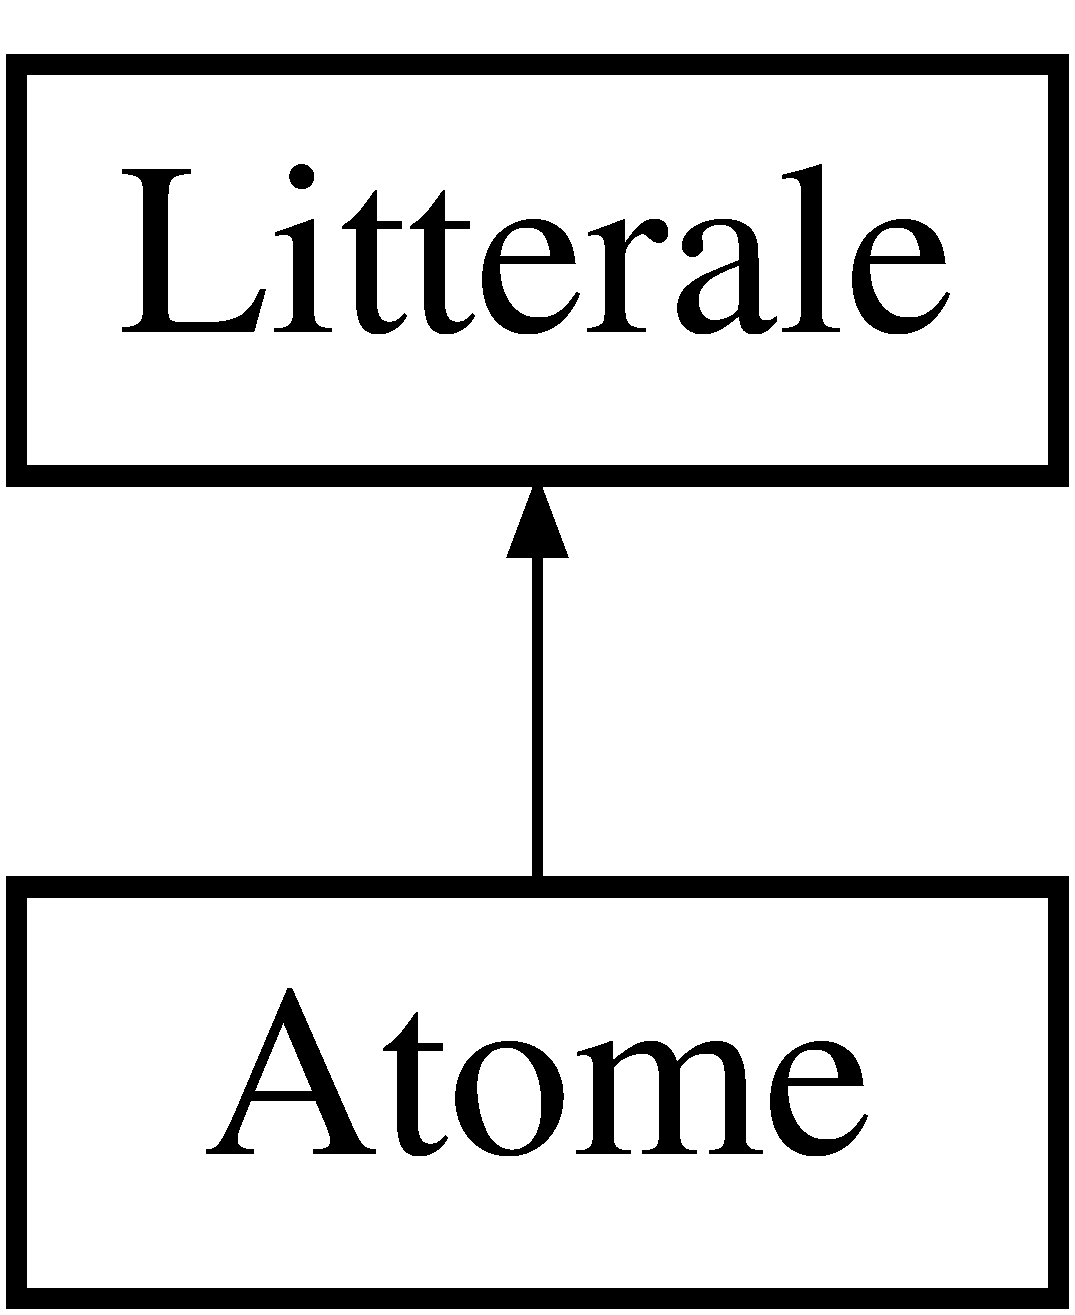
\includegraphics[height=2cm]{class_atome}
\end{center}
\end{figure}
\subsection*{Fonctions membres publiques}
\begin{CompactItemize}
\item 
\hypertarget{class_atome_8dfba20d5fba684abbd6be86d35744d5}{
\hyperlink{class_atome_8dfba20d5fba684abbd6be86d35744d5}{Atome} ()}
\label{class_atome_8dfba20d5fba684abbd6be86d35744d5}

\begin{CompactList}\small\item\em Constructeur. \item\end{CompactList}\item 
const string \hyperlink{class_atome_1ea077587e5f200c22bbec3784110452}{getId} () const 
\begin{CompactList}\small\item\em Accesseur. \item\end{CompactList}\item 
\hypertarget{class_atome_232aaac3d37c1d3d4acb6d6031e97e09}{
void \hyperlink{class_atome_232aaac3d37c1d3d4acb6d6031e97e09}{affiche} () const }
\label{class_atome_232aaac3d37c1d3d4acb6d6031e97e09}

\begin{CompactList}\small\item\em Redefinition de la fonction d'affichage. \item\end{CompactList}\item 
\hypertarget{class_atome_5cc14942990769be4455a1a4c813584d}{
\hyperlink{class_atome}{Atome} $\ast$ \hyperlink{class_atome_5cc14942990769be4455a1a4c813584d}{clone} ()}
\label{class_atome_5cc14942990769be4455a1a4c813584d}

\begin{CompactList}\small\item\em Redefinition de la fonction de clonage. \item\end{CompactList}\end{CompactItemize}


\subsection{Description détaillée}
Classe representant un atome, c'est a dire un identificateur (heritage de \hyperlink{class_litterale}{Litterale}). 

\subsection{Documentation des fonctions membres}
\hypertarget{class_atome_1ea077587e5f200c22bbec3784110452}{
\index{Atome@{Atome}!getId@{getId}}
\index{getId@{getId}!Atome@{Atome}}
\subsubsection[{getId}]{\setlength{\rightskip}{0pt plus 5cm}const string Atome::getId () const\hspace{0.3cm}{\tt  \mbox{[}inline\mbox{]}}}}
\label{class_atome_1ea077587e5f200c22bbec3784110452}


Accesseur. 

\begin{Desc}
\item[Renvoie:]chaine de caractere representant l'identifiant \end{Desc}


La documentation de cette classe a été générée à partir du fichier suivant :\begin{CompactItemize}
\item 
Litterale.h\end{CompactItemize}

\hypertarget{class_complexe}{
\section{Référence de la classe Complexe}
\label{class_complexe}\index{Complexe@{Complexe}}
}
Classe representant un nombre complexe (heritage de \hyperlink{class_litterale}{Litterale}).  


{\tt \#include $<$Litterale.h$>$}

Graphe d'héritage de Complexe::\begin{figure}[H]
\begin{center}
\leavevmode
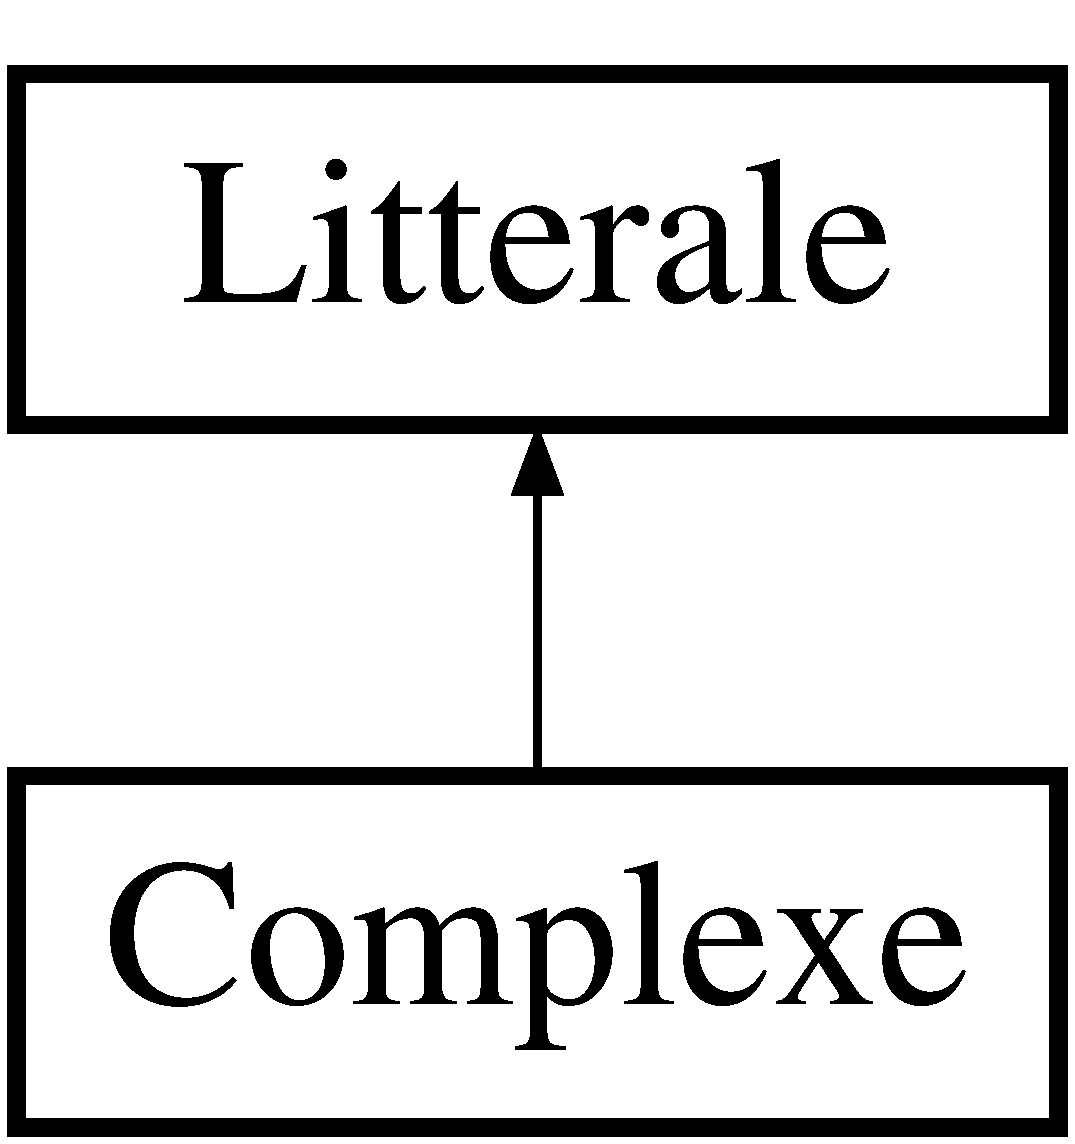
\includegraphics[height=2cm]{class_complexe}
\end{center}
\end{figure}
\subsection*{Fonctions membres publiques}
\begin{CompactItemize}
\item 
\hyperlink{class_complexe_bef2deb54a211490612383ce80657cb6}{Complexe} (\hyperlink{class_numerique}{Numerique} $\ast$r, \hyperlink{class_numerique}{Numerique} $\ast$i=nullptr)
\begin{CompactList}\small\item\em Constructeur. \item\end{CompactList}\item 
\hyperlink{class_numerique}{Numerique} $\ast$ \hyperlink{class_complexe_6485653e44cbffd188a219f9eb023311}{getRe} () const 
\begin{CompactList}\small\item\em Accesseur sur la partie reelle. \item\end{CompactList}\item 
\hyperlink{class_numerique}{Numerique} $\ast$ \hyperlink{class_complexe_116626f10f871db6145b197e392f22dd}{getIm} () const 
\begin{CompactList}\small\item\em Accesseur sur la partie imaginaire. \item\end{CompactList}\item 
\hypertarget{class_complexe_f55c7616e68169f79c26bf38be0318fe}{
void \hyperlink{class_complexe_f55c7616e68169f79c26bf38be0318fe}{affiche} () const }
\label{class_complexe_f55c7616e68169f79c26bf38be0318fe}

\begin{CompactList}\small\item\em Redefinition de la fonction d'affichage. \item\end{CompactList}\item 
\hypertarget{class_complexe_1dc5a5bc3559c7531e4c66f427164b71}{
\hyperlink{class_complexe}{Complexe} $\ast$ \hyperlink{class_complexe_1dc5a5bc3559c7531e4c66f427164b71}{clone} ()}
\label{class_complexe_1dc5a5bc3559c7531e4c66f427164b71}

\begin{CompactList}\small\item\em Redefinition de la fonction de clonage. \item\end{CompactList}\item 
\hypertarget{class_complexe_7496bd8781c9a32fff3b246bfb24b3c5}{
void \hyperlink{class_complexe_7496bd8781c9a32fff3b246bfb24b3c5}{neg} ()}
\label{class_complexe_7496bd8781c9a32fff3b246bfb24b3c5}

\begin{CompactList}\small\item\em Redefinition de la fonction d'inversion de signe. \item\end{CompactList}\end{CompactItemize}


\subsection{Description détaillée}
Classe representant un nombre complexe (heritage de \hyperlink{class_litterale}{Litterale}). 

\subsection{Documentation des constructeurs et destructeur}
\hypertarget{class_complexe_bef2deb54a211490612383ce80657cb6}{
\index{Complexe@{Complexe}!Complexe@{Complexe}}
\index{Complexe@{Complexe}!Complexe@{Complexe}}
\subsubsection[{Complexe}]{\setlength{\rightskip}{0pt plus 5cm}Complexe::Complexe ({\bf Numerique} $\ast$ {\em r}, \/  {\bf Numerique} $\ast$ {\em i} = {\tt nullptr})\hspace{0.3cm}{\tt  \mbox{[}inline\mbox{]}}}}
\label{class_complexe_bef2deb54a211490612383ce80657cb6}


Constructeur. 

\begin{Desc}
\item[Paramètres:]
\begin{description}
\item[{\em r}]: pointeur sur la litterale nuemerique representant la partie reelle \item[{\em i}]: pointeur sur la litterale nuemerique representant la partie imaginaire \end{description}
\end{Desc}


\subsection{Documentation des fonctions membres}
\hypertarget{class_complexe_116626f10f871db6145b197e392f22dd}{
\index{Complexe@{Complexe}!getIm@{getIm}}
\index{getIm@{getIm}!Complexe@{Complexe}}
\subsubsection[{getIm}]{\setlength{\rightskip}{0pt plus 5cm}{\bf Numerique}$\ast$ Complexe::getIm () const\hspace{0.3cm}{\tt  \mbox{[}inline\mbox{]}}}}
\label{class_complexe_116626f10f871db6145b197e392f22dd}


Accesseur sur la partie imaginaire. 

\begin{Desc}
\item[Renvoie:]valeur de la partie imaginaire du complexe (litterale numerique quelconque \end{Desc}
\hypertarget{class_complexe_6485653e44cbffd188a219f9eb023311}{
\index{Complexe@{Complexe}!getRe@{getRe}}
\index{getRe@{getRe}!Complexe@{Complexe}}
\subsubsection[{getRe}]{\setlength{\rightskip}{0pt plus 5cm}{\bf Numerique}$\ast$ Complexe::getRe () const\hspace{0.3cm}{\tt  \mbox{[}inline\mbox{]}}}}
\label{class_complexe_6485653e44cbffd188a219f9eb023311}


Accesseur sur la partie reelle. 

\begin{Desc}
\item[Renvoie:]valeur de la partie reelle du complexe (litterale numerique quelconque \end{Desc}


La documentation de cette classe a été générée à partir du fichier suivant :\begin{CompactItemize}
\item 
Litterale.h\end{CompactItemize}

\hypertarget{class_computer_exception}{
\section{Référence de la classe ComputerException}
\label{class_computer_exception}\index{ComputerException@{ComputerException}}
}
Classe permettant la gestion des erreurs.  


{\tt \#include $<$ComputerException.h$>$}

\subsection*{Fonctions membres publiques}
\begin{CompactItemize}
\item 
\hyperlink{class_computer_exception_99e174aa8c506b2f4d9bc3dc7846cc8a}{ComputerException} (const string \&str)
\begin{CompactList}\small\item\em Constructeur. \item\end{CompactList}\item 
string \hyperlink{class_computer_exception_a4c5726f929576598b204e162b6912fa}{getInfo} () const 
\begin{CompactList}\small\item\em Accesseur. \item\end{CompactList}\end{CompactItemize}


\subsection{Description détaillée}
Classe permettant la gestion des erreurs. 

\subsection{Documentation des constructeurs et destructeur}
\hypertarget{class_computer_exception_99e174aa8c506b2f4d9bc3dc7846cc8a}{
\index{ComputerException@{ComputerException}!ComputerException@{ComputerException}}
\index{ComputerException@{ComputerException}!ComputerException@{ComputerException}}
\subsubsection[{ComputerException}]{\setlength{\rightskip}{0pt plus 5cm}ComputerException::ComputerException (const string \& {\em str})\hspace{0.3cm}{\tt  \mbox{[}inline\mbox{]}}}}
\label{class_computer_exception_99e174aa8c506b2f4d9bc3dc7846cc8a}


Constructeur. 

\begin{Desc}
\item[Paramètres:]
\begin{description}
\item[{\em str}]: chaine de caracteres decrivant l'erreur \end{description}
\end{Desc}


\subsection{Documentation des fonctions membres}
\hypertarget{class_computer_exception_a4c5726f929576598b204e162b6912fa}{
\index{ComputerException@{ComputerException}!getInfo@{getInfo}}
\index{getInfo@{getInfo}!ComputerException@{ComputerException}}
\subsubsection[{getInfo}]{\setlength{\rightskip}{0pt plus 5cm}string ComputerException::getInfo () const\hspace{0.3cm}{\tt  \mbox{[}inline\mbox{]}}}}
\label{class_computer_exception_a4c5726f929576598b204e162b6912fa}


Accesseur. 

\begin{Desc}
\item[Renvoie:]chaine de caracteres decrivant l'erreur \end{Desc}


La documentation de cette classe a été générée à partir du fichier suivant :\begin{CompactItemize}
\item 
\hyperlink{_computer_exception_8h}{ComputerException.h}\end{CompactItemize}

\hypertarget{class_controleur}{
\section{Référence de la classe Controleur}
\label{class_controleur}\index{Controleur@{Controleur}}
}
Classe permettant de gerer l'ensemble de la calculatrice.  


{\tt \#include $<$Controleur.h$>$}

\subsection*{Fonctions membres publiques}
\begin{CompactItemize}
\item 
\hyperlink{class_controleur_b5ba4bff7cacbe4aaaa7f926cfb638f0}{Controleur} (\hyperlink{class_litterale_manager}{LitteraleManager} \&l, \hyperlink{class_pile}{Pile} \&v, \hyperlink{class_hash_map}{HashMap} \&t)
\begin{CompactList}\small\item\em Constructeur. \item\end{CompactList}\item 
void \hyperlink{class_controleur_3b3ae1907bbec700443d18ebed7c4131}{parse} (const string \&c)
\begin{CompactList}\small\item\em Parseur : permet d'analyser la chaine entree par l'utilisateur. \item\end{CompactList}\item 
\hypertarget{class_controleur_040d1f47fea94b243efc6040b0c105c0}{
void \hyperlink{class_controleur_040d1f47fea94b243efc6040b0c105c0}{executer} ()}
\label{class_controleur_040d1f47fea94b243efc6040b0c105c0}

\begin{CompactList}\small\item\em Lanceur : permet de lancer l'application. \item\end{CompactList}\item 
void \hyperlink{class_controleur_0b31c80009731bc370277e3ce62b6df7}{operation} (int i)
\begin{CompactList}\small\item\em Operation : permet d'effectuer des operations arithmetiques entre litterales. \item\end{CompactList}\item 
void \hyperlink{class_controleur_59c48ea6ab32a447c665ca1b7c220f8f}{operationPile} (int i)
\begin{CompactList}\small\item\em OperationPile : permet d'effectuer des operations directement sur la pile (DUP, SWAP, ...). \item\end{CompactList}\end{CompactItemize}
\subsection*{Attributs publics}
\begin{CompactItemize}
\item 
const int \hyperlink{class_controleur_bf929a8bcaec5e62b982c59d0a7f6166}{nbOpBin} = 8
\end{CompactItemize}


\subsection{Description détaillée}
Classe permettant de gerer l'ensemble de la calculatrice. 

\subsection{Documentation des constructeurs et destructeur}
\hypertarget{class_controleur_b5ba4bff7cacbe4aaaa7f926cfb638f0}{
\index{Controleur@{Controleur}!Controleur@{Controleur}}
\index{Controleur@{Controleur}!Controleur@{Controleur}}
\subsubsection[{Controleur}]{\setlength{\rightskip}{0pt plus 5cm}Controleur::Controleur ({\bf LitteraleManager} \& {\em l}, \/  {\bf Pile} \& {\em v}, \/  {\bf HashMap} \& {\em t})\hspace{0.3cm}{\tt  \mbox{[}inline\mbox{]}}}}
\label{class_controleur_b5ba4bff7cacbe4aaaa7f926cfb638f0}


Constructeur. 

\begin{Desc}
\item[Paramètres:]
\begin{description}
\item[{\em l}]: reference sur un litteraleManager \item[{\em v}]: reference sur une pile \item[{\em t}]: reference sur une hashmap \end{description}
\end{Desc}


\subsection{Documentation des fonctions membres}
\hypertarget{class_controleur_0b31c80009731bc370277e3ce62b6df7}{
\index{Controleur@{Controleur}!operation@{operation}}
\index{operation@{operation}!Controleur@{Controleur}}
\subsubsection[{operation}]{\setlength{\rightskip}{0pt plus 5cm}void Controleur::operation (int {\em i})}}
\label{class_controleur_0b31c80009731bc370277e3ce62b6df7}


Operation : permet d'effectuer des operations arithmetiques entre litterales. 

\begin{Desc}
\item[Paramètres:]
\begin{description}
\item[{\em i}]: un entier representant le type d'operation a realiser \end{description}
\end{Desc}
\hypertarget{class_controleur_59c48ea6ab32a447c665ca1b7c220f8f}{
\index{Controleur@{Controleur}!operationPile@{operationPile}}
\index{operationPile@{operationPile}!Controleur@{Controleur}}
\subsubsection[{operationPile}]{\setlength{\rightskip}{0pt plus 5cm}void Controleur::operationPile (int {\em i})}}
\label{class_controleur_59c48ea6ab32a447c665ca1b7c220f8f}


OperationPile : permet d'effectuer des operations directement sur la pile (DUP, SWAP, ...). 

\begin{Desc}
\item[Paramètres:]
\begin{description}
\item[{\em i}]: un entier representant le type d'operation a realiser \end{description}
\end{Desc}
\hypertarget{class_controleur_3b3ae1907bbec700443d18ebed7c4131}{
\index{Controleur@{Controleur}!parse@{parse}}
\index{parse@{parse}!Controleur@{Controleur}}
\subsubsection[{parse}]{\setlength{\rightskip}{0pt plus 5cm}void Controleur::parse (const string \& {\em c})}}
\label{class_controleur_3b3ae1907bbec700443d18ebed7c4131}


Parseur : permet d'analyser la chaine entree par l'utilisateur. 

$\ast$$\ast$$\ast$$\ast$$\ast$$\ast$Controleur$\ast$$\ast$$\ast$$\ast$$\ast$$\ast$/

\begin{Desc}
\item[Paramètres:]
\begin{description}
\item[{\em c}]: chaine de caracteres entree au clavier \end{description}
\end{Desc}


\subsection{Documentation des données membres}
\hypertarget{class_controleur_bf929a8bcaec5e62b982c59d0a7f6166}{
\index{Controleur@{Controleur}!nbOpBin@{nbOpBin}}
\index{nbOpBin@{nbOpBin}!Controleur@{Controleur}}
\subsubsection[{nbOpBin}]{\setlength{\rightskip}{0pt plus 5cm}const int {\bf Controleur::nbOpBin} = 8}}
\label{class_controleur_bf929a8bcaec5e62b982c59d0a7f6166}


Nombre d'operations binaires connues par le controleur 

La documentation de cette classe a été générée à partir des fichiers suivants :\begin{CompactItemize}
\item 
\hyperlink{_controleur_8h}{Controleur.h}\item 
Controleur.cpp\end{CompactItemize}

\hypertarget{class_entiere}{
\section{Référence de la classe Entiere}
\label{class_entiere}\index{Entiere@{Entiere}}
}
Classe representant un nombre entier (heritage de \hyperlink{class_numerique}{Numerique}).  


{\tt \#include $<$Litterale.h$>$}

Graphe d'héritage de Entiere::\begin{figure}[H]
\begin{center}
\leavevmode
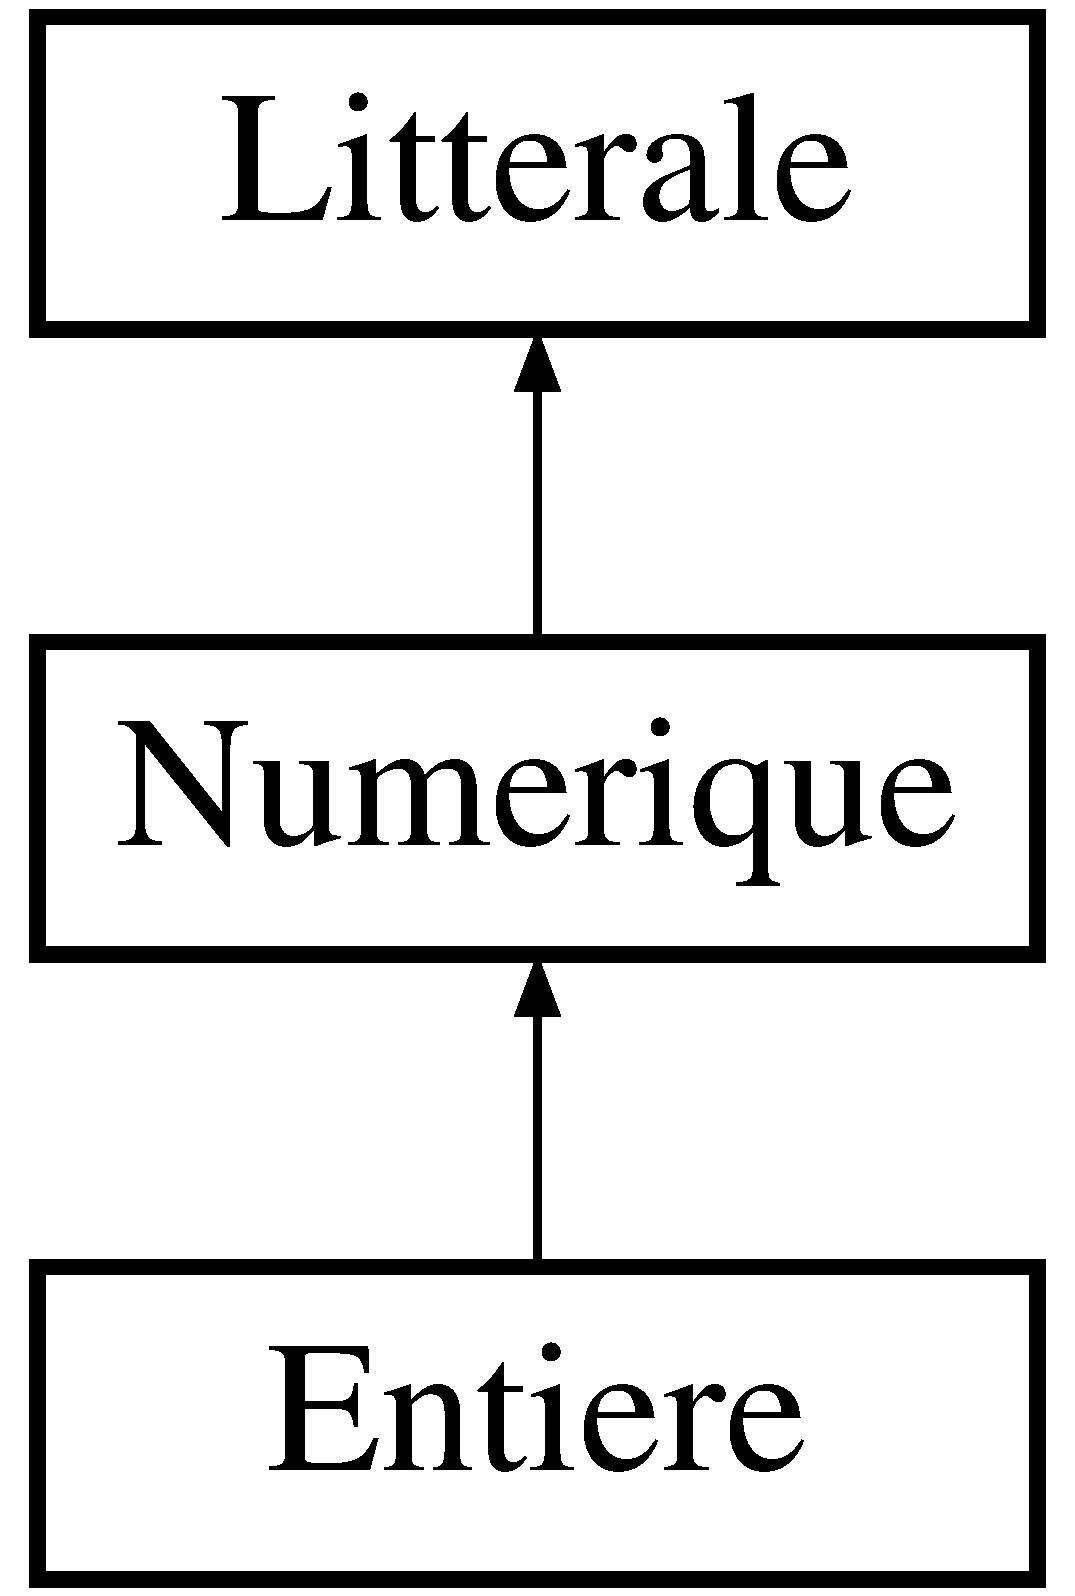
\includegraphics[height=3cm]{class_entiere}
\end{center}
\end{figure}
\subsection*{Fonctions membres publiques}
\begin{CompactItemize}
\item 
\hyperlink{class_entiere_ff8499408d074e26c267c2e1c6e696b8}{Entiere} (int v)
\begin{CompactList}\small\item\em Constructeur. \item\end{CompactList}\item 
int \hyperlink{class_entiere_d2517d3ce704cca0b13cfa0ee8c24cfd}{getVal} () const 
\begin{CompactList}\small\item\em Accesseur. \item\end{CompactList}\item 
\hypertarget{class_entiere_58d2569469b5d4765d815be15171a041}{
void \hyperlink{class_entiere_58d2569469b5d4765d815be15171a041}{affiche} () const }
\label{class_entiere_58d2569469b5d4765d815be15171a041}

\begin{CompactList}\small\item\em Redefinition de la fonction d'affichage. \item\end{CompactList}\item 
\hypertarget{class_entiere_bb972ef0ad74814e4abf22c0cd3a2b55}{
void \hyperlink{class_entiere_bb972ef0ad74814e4abf22c0cd3a2b55}{neg} ()}
\label{class_entiere_bb972ef0ad74814e4abf22c0cd3a2b55}

\begin{CompactList}\small\item\em Redefinition de la fonction d'inversion de signe. \item\end{CompactList}\item 
void \hyperlink{class_entiere_c3dae32e641989e217776e93005ec570}{setVal} (int i)
\begin{CompactList}\small\item\em Editeur : permet de modifier la valeur de la litterale. \item\end{CompactList}\item 
\hypertarget{class_entiere_94592b044a5bee1b5c2ef5e6b3fd8e64}{
\hyperlink{class_entiere}{Entiere} $\ast$ \hyperlink{class_entiere_94592b044a5bee1b5c2ef5e6b3fd8e64}{clone} ()}
\label{class_entiere_94592b044a5bee1b5c2ef5e6b3fd8e64}

\begin{CompactList}\small\item\em Redefinition de la fonction de clonage. \item\end{CompactList}\item 
\hypertarget{class_entiere_7215a91e24996f79640e766e660907cc}{
double \hyperlink{class_entiere_7215a91e24996f79640e766e660907cc}{getComp} ()}
\label{class_entiere_7215a91e24996f79640e766e660907cc}

\begin{CompactList}\small\item\em Redefinition de la fonction de comparaison. \item\end{CompactList}\end{CompactItemize}


\subsection{Description détaillée}
Classe representant un nombre entier (heritage de \hyperlink{class_numerique}{Numerique}). 

\subsection{Documentation des constructeurs et destructeur}
\hypertarget{class_entiere_ff8499408d074e26c267c2e1c6e696b8}{
\index{Entiere@{Entiere}!Entiere@{Entiere}}
\index{Entiere@{Entiere}!Entiere@{Entiere}}
\subsubsection[{Entiere}]{\setlength{\rightskip}{0pt plus 5cm}Entiere::Entiere (int {\em v})\hspace{0.3cm}{\tt  \mbox{[}inline\mbox{]}}}}
\label{class_entiere_ff8499408d074e26c267c2e1c6e696b8}


Constructeur. 

\begin{Desc}
\item[Paramètres:]
\begin{description}
\item[{\em v}]: entier representant la valeur de la litterale \end{description}
\end{Desc}


\subsection{Documentation des fonctions membres}
\hypertarget{class_entiere_d2517d3ce704cca0b13cfa0ee8c24cfd}{
\index{Entiere@{Entiere}!getVal@{getVal}}
\index{getVal@{getVal}!Entiere@{Entiere}}
\subsubsection[{getVal}]{\setlength{\rightskip}{0pt plus 5cm}int Entiere::getVal () const\hspace{0.3cm}{\tt  \mbox{[}inline\mbox{]}}}}
\label{class_entiere_d2517d3ce704cca0b13cfa0ee8c24cfd}


Accesseur. 

\begin{Desc}
\item[Renvoie:]s : entier representant la valeur de la litterale \end{Desc}
\hypertarget{class_entiere_c3dae32e641989e217776e93005ec570}{
\index{Entiere@{Entiere}!setVal@{setVal}}
\index{setVal@{setVal}!Entiere@{Entiere}}
\subsubsection[{setVal}]{\setlength{\rightskip}{0pt plus 5cm}void Entiere::setVal (int {\em i})\hspace{0.3cm}{\tt  \mbox{[}inline\mbox{]}}}}
\label{class_entiere_c3dae32e641989e217776e93005ec570}


Editeur : permet de modifier la valeur de la litterale. 

\begin{Desc}
\item[Paramètres:]
\begin{description}
\item[{\em i}]: entier representant la nouvelle valeur de la litterale \end{description}
\end{Desc}


La documentation de cette classe a été générée à partir du fichier suivant :\begin{CompactItemize}
\item 
Litterale.h\end{CompactItemize}

\hypertarget{class_expression}{
\section{Référence de la classe Expression}
\label{class_expression}\index{Expression@{Expression}}
}
Classe representant une expression, c'est a dire une suite d'operations (heritage de \hyperlink{class_litterale}{Litterale}).  


{\tt \#include $<$Litterale.h$>$}

Graphe d'héritage de Expression::\begin{figure}[H]
\begin{center}
\leavevmode
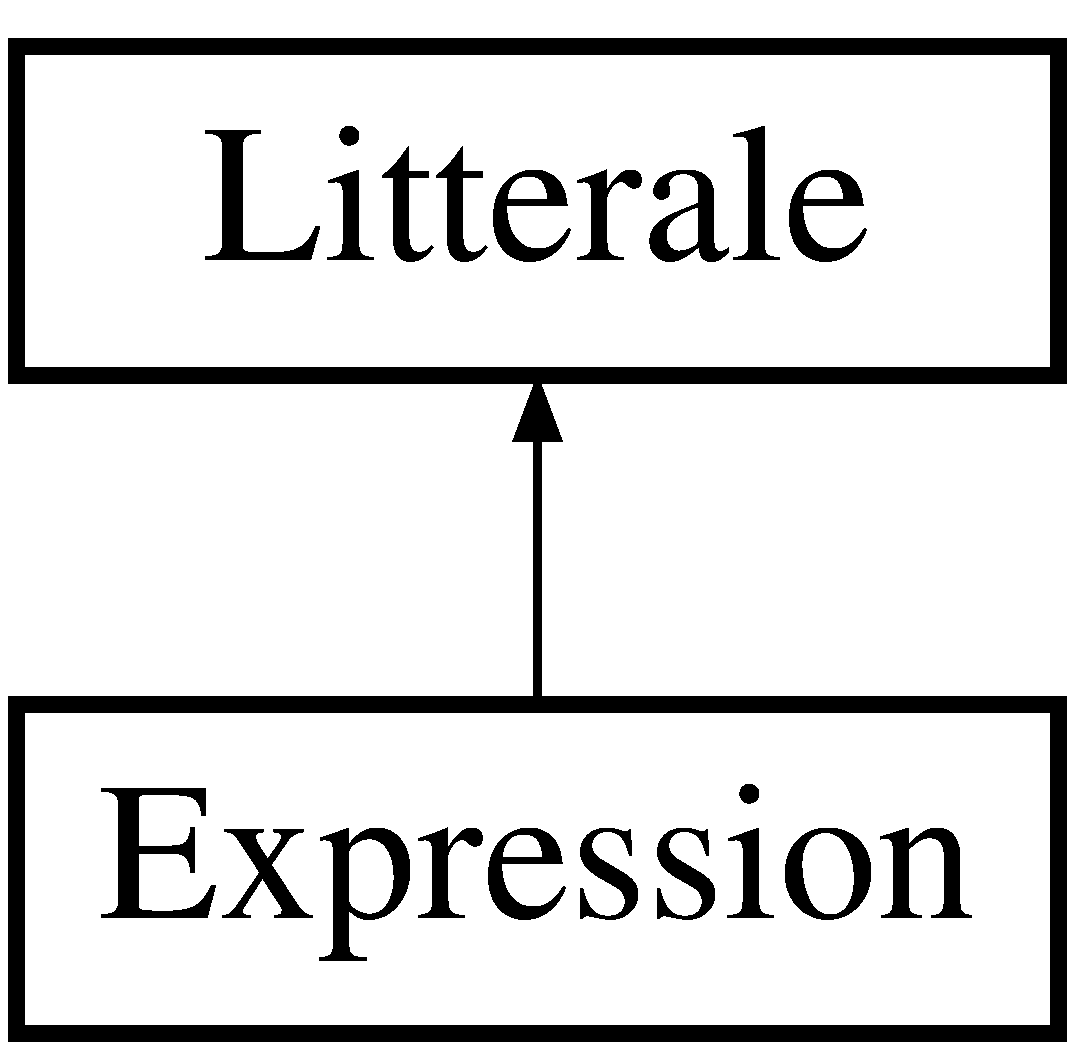
\includegraphics[height=2cm]{class_expression}
\end{center}
\end{figure}
\subsection*{Fonctions membres publiques}
\begin{CompactItemize}
\item 
\hyperlink{class_expression_63fded6eef43b0507d9d2bd4c7fae0f9}{Expression} (string s)
\begin{CompactList}\small\item\em Constructeur. \item\end{CompactList}\item 
const string \hyperlink{class_expression_392af96c64d27d5aa23bc3993fa40a62}{getExpr} () const 
\begin{CompactList}\small\item\em Accesseur. \item\end{CompactList}\item 
\hypertarget{class_expression_a061cfda7d2152ebb166ec86258dc059}{
void \hyperlink{class_expression_a061cfda7d2152ebb166ec86258dc059}{affiche} () const }
\label{class_expression_a061cfda7d2152ebb166ec86258dc059}

\begin{CompactList}\small\item\em Redefinition de la fonction d'affichage. \item\end{CompactList}\item 
\hypertarget{class_expression_5f81067f280c6419d8bd0b117a2d6f13}{
\hyperlink{class_expression}{Expression} $\ast$ \hyperlink{class_expression_5f81067f280c6419d8bd0b117a2d6f13}{clone} ()}
\label{class_expression_5f81067f280c6419d8bd0b117a2d6f13}

\begin{CompactList}\small\item\em Redefinition de la fonction de clonage. \item\end{CompactList}\end{CompactItemize}


\subsection{Description détaillée}
Classe representant une expression, c'est a dire une suite d'operations (heritage de \hyperlink{class_litterale}{Litterale}). 

\subsection{Documentation des constructeurs et destructeur}
\hypertarget{class_expression_63fded6eef43b0507d9d2bd4c7fae0f9}{
\index{Expression@{Expression}!Expression@{Expression}}
\index{Expression@{Expression}!Expression@{Expression}}
\subsubsection[{Expression}]{\setlength{\rightskip}{0pt plus 5cm}Expression::Expression (string {\em s})\hspace{0.3cm}{\tt  \mbox{[}inline\mbox{]}}}}
\label{class_expression_63fded6eef43b0507d9d2bd4c7fae0f9}


Constructeur. 

\begin{Desc}
\item[Paramètres:]
\begin{description}
\item[{\em s}]: chaine de caractere representant le contenu de l'expression \end{description}
\end{Desc}


\subsection{Documentation des fonctions membres}
\hypertarget{class_expression_392af96c64d27d5aa23bc3993fa40a62}{
\index{Expression@{Expression}!getExpr@{getExpr}}
\index{getExpr@{getExpr}!Expression@{Expression}}
\subsubsection[{getExpr}]{\setlength{\rightskip}{0pt plus 5cm}const string Expression::getExpr () const\hspace{0.3cm}{\tt  \mbox{[}inline\mbox{]}}}}
\label{class_expression_392af96c64d27d5aa23bc3993fa40a62}


Accesseur. 

\begin{Desc}
\item[Renvoie:]chaine de caractere representant le contenu de l'expression \end{Desc}


La documentation de cette classe a été générée à partir du fichier suivant :\begin{CompactItemize}
\item 
Litterale.h\end{CompactItemize}

\hypertarget{class_hash_entry}{
\section{Référence de la classe HashEntry}
\label{class_hash_entry}\index{HashEntry@{HashEntry}}
}
Classe representant une entree de la \hyperlink{class_hash_map}{HashMap}.  


{\tt \#include $<$HashMap.h$>$}

\subsection*{Fonctions membres publiques}
\begin{CompactItemize}
\item 
\hyperlink{class_hash_entry_14144ea0077dd77f83ec2be03c019033}{HashEntry} (string key, \hyperlink{class_litterale}{Litterale} $\ast$value)
\begin{CompactList}\small\item\em Constructeur. \item\end{CompactList}\item 
string \hyperlink{class_hash_entry_040b7d2f3147a6944ad8d66301bdf80d}{getKey} ()
\begin{CompactList}\small\item\em Accesseur. \item\end{CompactList}\item 
\hyperlink{class_litterale}{Litterale} $\ast$ \hyperlink{class_hash_entry_0edc1c3f8c73882a6d8a9fec88c45f6b}{getValue} ()
\begin{CompactList}\small\item\em Accesseur. \item\end{CompactList}\end{CompactItemize}


\subsection{Description détaillée}
Classe representant une entree de la \hyperlink{class_hash_map}{HashMap}. 

\subsection{Documentation des constructeurs et destructeur}
\hypertarget{class_hash_entry_14144ea0077dd77f83ec2be03c019033}{
\index{HashEntry@{HashEntry}!HashEntry@{HashEntry}}
\index{HashEntry@{HashEntry}!HashEntry@{HashEntry}}
\subsubsection[{HashEntry}]{\setlength{\rightskip}{0pt plus 5cm}HashEntry::HashEntry (string {\em key}, \/  {\bf Litterale} $\ast$ {\em value})\hspace{0.3cm}{\tt  \mbox{[}inline\mbox{]}}}}
\label{class_hash_entry_14144ea0077dd77f83ec2be03c019033}


Constructeur. 

\begin{Desc}
\item[Paramètres:]
\begin{description}
\item[{\em key}]: chaine de caracteres servant d'identifiant a la variable ou au programme \item[{\em value}]: pointeur sur la litterale stockee \end{description}
\end{Desc}


\subsection{Documentation des fonctions membres}
\hypertarget{class_hash_entry_040b7d2f3147a6944ad8d66301bdf80d}{
\index{HashEntry@{HashEntry}!getKey@{getKey}}
\index{getKey@{getKey}!HashEntry@{HashEntry}}
\subsubsection[{getKey}]{\setlength{\rightskip}{0pt plus 5cm}string HashEntry::getKey ()\hspace{0.3cm}{\tt  \mbox{[}inline\mbox{]}}}}
\label{class_hash_entry_040b7d2f3147a6944ad8d66301bdf80d}


Accesseur. 

\begin{Desc}
\item[Renvoie:]chaine caracteres servant d'identifiant a la variable ou au programme \end{Desc}
\hypertarget{class_hash_entry_0edc1c3f8c73882a6d8a9fec88c45f6b}{
\index{HashEntry@{HashEntry}!getValue@{getValue}}
\index{getValue@{getValue}!HashEntry@{HashEntry}}
\subsubsection[{getValue}]{\setlength{\rightskip}{0pt plus 5cm}{\bf Litterale}$\ast$ HashEntry::getValue ()\hspace{0.3cm}{\tt  \mbox{[}inline\mbox{]}}}}
\label{class_hash_entry_0edc1c3f8c73882a6d8a9fec88c45f6b}


Accesseur. 

\begin{Desc}
\item[Renvoie:]pointeur sur la litterale stockee \end{Desc}


La documentation de cette classe a été générée à partir du fichier suivant :\begin{CompactItemize}
\item 
HashMap.h\end{CompactItemize}

\hypertarget{class_hash_map}{
\section{Référence de la classe HashMap}
\label{class_hash_map}\index{HashMap@{HashMap}}
}
Classe reprentant la table de stockage.  


{\tt \#include $<$HashMap.h$>$}

\subsection*{Fonctions membres publiques}
\begin{CompactItemize}
\item 
\hypertarget{class_hash_map_3ae91705aa3ebfff22ce92e3c7797050}{
\hyperlink{class_hash_map_3ae91705aa3ebfff22ce92e3c7797050}{HashMap} ()}
\label{class_hash_map_3ae91705aa3ebfff22ce92e3c7797050}

\begin{CompactList}\small\item\em Constructeur. \item\end{CompactList}\item 
\hyperlink{class_litterale}{Litterale} $\ast$ \hyperlink{class_hash_map_28d6dfc1112eb216a754c07255ce0ba3}{get} (string key)
\begin{CompactList}\small\item\em Accesseur dans la table. \item\end{CompactList}\item 
void \hyperlink{class_hash_map_79196be9d74f1da3c2985e19c50e4790}{put} (string key, \hyperlink{class_litterale}{Litterale} $\ast$value)
\begin{CompactList}\small\item\em Ajout d'une entree dans la table. \item\end{CompactList}\item 
void \hyperlink{class_hash_map_32fb1e4adb8f3982861772efa511f7db}{forget} (string key)
\begin{CompactList}\small\item\em Oubli d'une entree de la table. \item\end{CompactList}\item 
\hypertarget{class_hash_map_7120321a936e8018fd276bcd4b4da3b8}{
\hyperlink{class_hash_map_7120321a936e8018fd276bcd4b4da3b8}{$\sim$HashMap} ()}
\label{class_hash_map_7120321a936e8018fd276bcd4b4da3b8}

\begin{CompactList}\small\item\em Destructeur. \item\end{CompactList}\end{CompactItemize}


\subsection{Description détaillée}
Classe reprentant la table de stockage. 

\subsection{Documentation des fonctions membres}
\hypertarget{class_hash_map_32fb1e4adb8f3982861772efa511f7db}{
\index{HashMap@{HashMap}!forget@{forget}}
\index{forget@{forget}!HashMap@{HashMap}}
\subsubsection[{forget}]{\setlength{\rightskip}{0pt plus 5cm}void HashMap::forget (string {\em key})\hspace{0.3cm}{\tt  \mbox{[}inline\mbox{]}}}}
\label{class_hash_map_32fb1e4adb8f3982861772efa511f7db}


Oubli d'une entree de la table. 

\begin{Desc}
\item[Paramètres:]
\begin{description}
\item[{\em key}]: chaine de caracteres servant d'identifiant a la variable ou au programme \end{description}
\end{Desc}
\hypertarget{class_hash_map_28d6dfc1112eb216a754c07255ce0ba3}{
\index{HashMap@{HashMap}!get@{get}}
\index{get@{get}!HashMap@{HashMap}}
\subsubsection[{get}]{\setlength{\rightskip}{0pt plus 5cm}{\bf Litterale}$\ast$ HashMap::get (string {\em key})\hspace{0.3cm}{\tt  \mbox{[}inline\mbox{]}}}}
\label{class_hash_map_28d6dfc1112eb216a754c07255ce0ba3}


Accesseur dans la table. 

\begin{Desc}
\item[Paramètres:]
\begin{description}
\item[{\em key}]: chaine de caracteres servant d'identifiant a la variable ou au programme dont on cherche la valeur \end{description}
\end{Desc}
\begin{Desc}
\item[Renvoie:]pointeur sur la litterale correspondante \end{Desc}
\hypertarget{class_hash_map_79196be9d74f1da3c2985e19c50e4790}{
\index{HashMap@{HashMap}!put@{put}}
\index{put@{put}!HashMap@{HashMap}}
\subsubsection[{put}]{\setlength{\rightskip}{0pt plus 5cm}void HashMap::put (string {\em key}, \/  {\bf Litterale} $\ast$ {\em value})\hspace{0.3cm}{\tt  \mbox{[}inline\mbox{]}}}}
\label{class_hash_map_79196be9d74f1da3c2985e19c50e4790}


Ajout d'une entree dans la table. 

\begin{Desc}
\item[Paramètres:]
\begin{description}
\item[{\em key}]: chaine de caracteres servant d'identifiant a la variable ou au programme a inserer \item[{\em value}]: pointeur sur la litterale correspondante a inserer \end{description}
\end{Desc}


La documentation de cette classe a été générée à partir du fichier suivant :\begin{CompactItemize}
\item 
HashMap.h\end{CompactItemize}

\hypertarget{class_item}{
\section{Référence de la classe Item}
\label{class_item}\index{Item@{Item}}
}
Classe permettant d'encapsuler les litterales dans des items pour le stockage dans la pile.  


{\tt \#include $<$Pile.h$>$}

\subsection*{Fonctions membres publiques}
\begin{CompactItemize}
\item 
\hypertarget{class_item_297720c02984eab37332ae795d22189d}{
\hyperlink{class_item_297720c02984eab37332ae795d22189d}{Item} ()}
\label{class_item_297720c02984eab37332ae795d22189d}

\begin{CompactList}\small\item\em Constructeur. \item\end{CompactList}\item 
void \hyperlink{class_item_0c2c0a79074c81befa8d1956636cd67d}{setLitterale} (\hyperlink{class_litterale}{Litterale} $\ast$const l)
\begin{CompactList}\small\item\em Editeur : permet de changer la litterale pointee. \item\end{CompactList}\item 
\hyperlink{class_litterale}{Litterale} $\ast$const \hyperlink{class_item_128005ee69ac247ac82460c21f85ce3f}{getLitterale} () const 
\begin{CompactList}\small\item\em Accesseur. \item\end{CompactList}\item 
\hypertarget{class_item_24858085cb6b69b1776423bc9a6ce4ce}{
void \hyperlink{class_item_24858085cb6b69b1776423bc9a6ce4ce}{raz} ()}
\label{class_item_24858085cb6b69b1776423bc9a6ce4ce}

\begin{CompactList}\small\item\em Reset de l'item. \item\end{CompactList}\end{CompactItemize}


\subsection{Description détaillée}
Classe permettant d'encapsuler les litterales dans des items pour le stockage dans la pile. 

\subsection{Documentation des fonctions membres}
\hypertarget{class_item_128005ee69ac247ac82460c21f85ce3f}{
\index{Item@{Item}!getLitterale@{getLitterale}}
\index{getLitterale@{getLitterale}!Item@{Item}}
\subsubsection[{getLitterale}]{\setlength{\rightskip}{0pt plus 5cm}{\bf Litterale}$\ast$ const Item::getLitterale () const\hspace{0.3cm}{\tt  \mbox{[}inline\mbox{]}}}}
\label{class_item_128005ee69ac247ac82460c21f85ce3f}


Accesseur. 

\begin{Desc}
\item[Renvoie:]litterale pointee par l'item \end{Desc}
\hypertarget{class_item_0c2c0a79074c81befa8d1956636cd67d}{
\index{Item@{Item}!setLitterale@{setLitterale}}
\index{setLitterale@{setLitterale}!Item@{Item}}
\subsubsection[{setLitterale}]{\setlength{\rightskip}{0pt plus 5cm}void Item::setLitterale ({\bf Litterale} $\ast$const  {\em l})\hspace{0.3cm}{\tt  \mbox{[}inline\mbox{]}}}}
\label{class_item_0c2c0a79074c81befa8d1956636cd67d}


Editeur : permet de changer la litterale pointee. 

\begin{Desc}
\item[Paramètres:]
\begin{description}
\item[{\em l}]: pointeur sur la nouvelle litterale \end{description}
\end{Desc}


La documentation de cette classe a été générée à partir du fichier suivant :\begin{CompactItemize}
\item 
Pile.h\end{CompactItemize}

\hypertarget{class_litterale}{
\section{Référence de la classe Litterale}
\label{class_litterale}\index{Litterale@{Litterale}}
}
Classe abstraite representant toutes les litterales pouvant etres stockees.  


{\tt \#include $<$Litterale.h$>$}

Graphe d'héritage de Litterale::\begin{figure}[H]
\begin{center}
\leavevmode
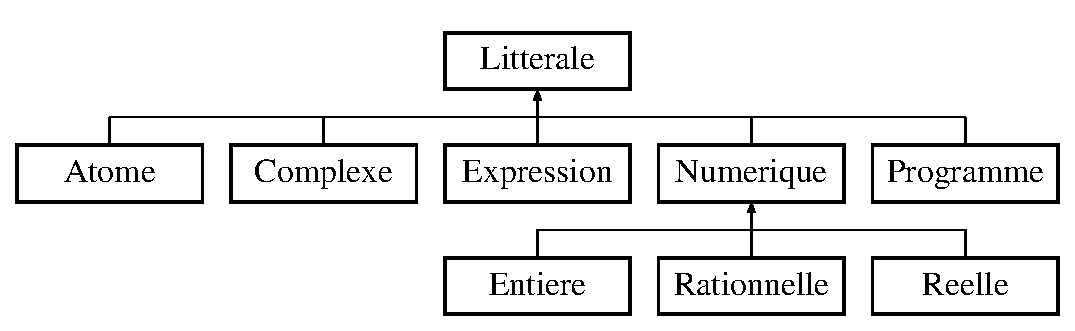
\includegraphics[height=3cm]{class_litterale}
\end{center}
\end{figure}
\subsection*{Fonctions membres publiques}
\begin{CompactItemize}
\item 
\hypertarget{class_litterale_a0a02717ec75f502f1afdb6ac597efac}{
\hyperlink{class_litterale_a0a02717ec75f502f1afdb6ac597efac}{Litterale} ()}
\label{class_litterale_a0a02717ec75f502f1afdb6ac597efac}

\begin{CompactList}\small\item\em Constructeur. \item\end{CompactList}\item 
\hypertarget{class_litterale_d67121b10b76b2283940c52cb3b26185}{
virtual void \hyperlink{class_litterale_d67121b10b76b2283940c52cb3b26185}{affiche} () const =0}
\label{class_litterale_d67121b10b76b2283940c52cb3b26185}

\begin{CompactList}\small\item\em Affiche : Methode virtuelle pure pour l'affichage d'une litterale. \item\end{CompactList}\item 
TypeLitterale \hyperlink{class_litterale_a974ab68a06e8a8b15d04ecd4ce8065a}{getType} () const 
\begin{CompactList}\small\item\em Accesseur. \item\end{CompactList}\item 
\hypertarget{class_litterale_aaadc01ca2bb0c9210f9de083130768b}{
virtual \hyperlink{class_litterale}{Litterale} $\ast$ \hyperlink{class_litterale_aaadc01ca2bb0c9210f9de083130768b}{clone} ()=0}
\label{class_litterale_aaadc01ca2bb0c9210f9de083130768b}

\begin{CompactList}\small\item\em Clone : Methode virtuelle pure permettant de dupliquer un pointeur sur litterale. \item\end{CompactList}\item 
\hypertarget{class_litterale_257dc6d6f3c4d8458d45be92ceede634}{
bool \hyperlink{class_litterale_257dc6d6f3c4d8458d45be92ceede634}{operator==} (\hyperlink{class_litterale}{Litterale} $\ast$l)}
\label{class_litterale_257dc6d6f3c4d8458d45be92ceede634}

\begin{CompactList}\small\item\em Surchage operateur==. \item\end{CompactList}\item 
\hypertarget{class_litterale_eae743dc3e6055579ec749b708c57bc9}{
bool \hyperlink{class_litterale_eae743dc3e6055579ec749b708c57bc9}{operator!=} (\hyperlink{class_litterale}{Litterale} $\ast$l)}
\label{class_litterale_eae743dc3e6055579ec749b708c57bc9}

\begin{CompactList}\small\item\em Surchage operateur!=. \item\end{CompactList}\item 
\hypertarget{class_litterale_b88999156adbab96ea31e255dd3da85d}{
bool \hyperlink{class_litterale_b88999156adbab96ea31e255dd3da85d}{operator$<$} (\hyperlink{class_litterale}{Litterale} $\ast$l)}
\label{class_litterale_b88999156adbab96ea31e255dd3da85d}

\begin{CompactList}\small\item\em Surchage operateur$<$. \item\end{CompactList}\item 
\hypertarget{class_litterale_3495fcc6429947a6625a11e0afa0b9c6}{
bool \hyperlink{class_litterale_3495fcc6429947a6625a11e0afa0b9c6}{operator$>$} (\hyperlink{class_litterale}{Litterale} $\ast$l)}
\label{class_litterale_3495fcc6429947a6625a11e0afa0b9c6}

\begin{CompactList}\small\item\em Surchage operateur$>$. \item\end{CompactList}\item 
\hypertarget{class_litterale_76f566c89aa02934839f159f8d627021}{
bool \hyperlink{class_litterale_76f566c89aa02934839f159f8d627021}{operator$<$=} (\hyperlink{class_litterale}{Litterale} $\ast$l)}
\label{class_litterale_76f566c89aa02934839f159f8d627021}

\begin{CompactList}\small\item\em Surchage operateur$<$=. \item\end{CompactList}\item 
\hypertarget{class_litterale_4a4dfdd26a03ecd6c38d1f7e6521b549}{
bool \hyperlink{class_litterale_4a4dfdd26a03ecd6c38d1f7e6521b549}{operator$>$=} (\hyperlink{class_litterale}{Litterale} $\ast$l)}
\label{class_litterale_4a4dfdd26a03ecd6c38d1f7e6521b549}

\begin{CompactList}\small\item\em Surchage operateur$>$=. \item\end{CompactList}\end{CompactItemize}
\subsection*{Attributs protégés}
\begin{CompactItemize}
\item 
TypeLitterale \hyperlink{class_litterale_ab5099a9b2acefce3bc3da9487e0ad78}{type}
\end{CompactItemize}


\subsection{Description détaillée}
Classe abstraite representant toutes les litterales pouvant etres stockees. 

\subsection{Documentation des fonctions membres}
\hypertarget{class_litterale_a974ab68a06e8a8b15d04ecd4ce8065a}{
\index{Litterale@{Litterale}!getType@{getType}}
\index{getType@{getType}!Litterale@{Litterale}}
\subsubsection[{getType}]{\setlength{\rightskip}{0pt plus 5cm}TypeLitterale Litterale::getType () const\hspace{0.3cm}{\tt  \mbox{[}inline\mbox{]}}}}
\label{class_litterale_a974ab68a06e8a8b15d04ecd4ce8065a}


Accesseur. 

\begin{Desc}
\item[Renvoie:]value : type precis de la litterale correspondant a un element d'une liste enumeree \end{Desc}


\subsection{Documentation des données membres}
\hypertarget{class_litterale_ab5099a9b2acefce3bc3da9487e0ad78}{
\index{Litterale@{Litterale}!type@{type}}
\index{type@{type}!Litterale@{Litterale}}
\subsubsection[{type}]{\setlength{\rightskip}{0pt plus 5cm}TypeLitterale {\bf Litterale::type}\hspace{0.3cm}{\tt  \mbox{[}protected\mbox{]}}}}
\label{class_litterale_ab5099a9b2acefce3bc3da9487e0ad78}


type precis de la litterale correspondant a un element d'une liste enumeree 

La documentation de cette classe a été générée à partir des fichiers suivants :\begin{CompactItemize}
\item 
Litterale.h\item 
Litterale.cpp\end{CompactItemize}

\hypertarget{class_litterale_manager}{
\section{Référence de la classe LitteraleManager}
\label{class_litterale_manager}\index{LitteraleManager@{LitteraleManager}}
}
Classe permettant de gerer toutes les litterales ajoutees une a une.  


{\tt \#include $<$LitteraleManager.h$>$}

\subsection*{Fonctions membres publiques}
\begin{CompactItemize}
\item 
\hypertarget{class_litterale_manager_daa9e81e06b8001e4cf9e0f5a214b6cd}{
\hyperlink{class_litterale_manager_daa9e81e06b8001e4cf9e0f5a214b6cd}{LitteraleManager} ()}
\label{class_litterale_manager_daa9e81e06b8001e4cf9e0f5a214b6cd}

\begin{CompactList}\small\item\em Constructeur. \item\end{CompactList}\item 
\hypertarget{class_litterale_manager_a6f690e84ae96ec3a15f6b629264cc1f}{
\hyperlink{class_litterale_manager_a6f690e84ae96ec3a15f6b629264cc1f}{$\sim$LitteraleManager} ()}
\label{class_litterale_manager_a6f690e84ae96ec3a15f6b629264cc1f}

\begin{CompactList}\small\item\em Destructeur. \item\end{CompactList}\item 
\hyperlink{class_litterale}{Litterale} \& \hyperlink{class_litterale_manager_bfb29c7c9e5ffdd6904f069def98d2df}{addLitterale} (\hyperlink{class_litterale}{Litterale} $\ast$const l)
\begin{CompactList}\small\item\em Ajout d'une litterale dans le Manager. \item\end{CompactList}\item 
\hyperlink{class_litterale}{Litterale} $\ast$const \hyperlink{class_litterale_manager_ac254ffc8158f21899786e2133a6018d}{littFactory} (TypeLitterale type, int p1, int p2=NULL, double p3=NULL, \hyperlink{class_numerique}{Numerique} $\ast$p4=nullptr, \hyperlink{class_numerique}{Numerique} $\ast$p5=nullptr)
\begin{CompactList}\small\item\em Creation de la litterale corespondant a la chaine de caracteres parsee dans le controleur. \item\end{CompactList}\item 
void \hyperlink{class_litterale_manager_53bfb9871eed94f6c3e8f5f1e2a76e29}{removeLitterale} (\hyperlink{class_litterale}{Litterale} $\ast$const l)
\begin{CompactList}\small\item\em Suppression d'une litterale du Manager. \item\end{CompactList}\end{CompactItemize}


\subsection{Description détaillée}
Classe permettant de gerer toutes les litterales ajoutees une a une. 

\subsection{Documentation des fonctions membres}
\hypertarget{class_litterale_manager_bfb29c7c9e5ffdd6904f069def98d2df}{
\index{LitteraleManager@{LitteraleManager}!addLitterale@{addLitterale}}
\index{addLitterale@{addLitterale}!LitteraleManager@{LitteraleManager}}
\subsubsection[{addLitterale}]{\setlength{\rightskip}{0pt plus 5cm}{\bf Litterale} \& LitteraleManager::addLitterale ({\bf Litterale} $\ast$const  {\em l})}}
\label{class_litterale_manager_bfb29c7c9e5ffdd6904f069def98d2df}


Ajout d'une litterale dans le Manager. 

\begin{Desc}
\item[Paramètres:]
\begin{description}
\item[{\em l}]: litterale a ajouter \end{description}
\end{Desc}
\begin{Desc}
\item[Renvoie:]reference sur la litterale ajoutee \end{Desc}
\hypertarget{class_litterale_manager_ac254ffc8158f21899786e2133a6018d}{
\index{LitteraleManager@{LitteraleManager}!littFactory@{littFactory}}
\index{littFactory@{littFactory}!LitteraleManager@{LitteraleManager}}
\subsubsection[{littFactory}]{\setlength{\rightskip}{0pt plus 5cm}{\bf Litterale} $\ast$const LitteraleManager::littFactory (TypeLitterale {\em type}, \/  int {\em p1}, \/  int {\em p2} = {\tt NULL}, \/  double {\em p3} = {\tt NULL}, \/  {\bf Numerique} $\ast$ {\em p4} = {\tt nullptr}, \/  {\bf Numerique} $\ast$ {\em p5} = {\tt nullptr})}}
\label{class_litterale_manager_ac254ffc8158f21899786e2133a6018d}


Creation de la litterale corespondant a la chaine de caracteres parsee dans le controleur. 

\begin{Desc}
\item[Paramètres:]
\begin{description}
\item[{\em type}]: type precis de la litterale a creer \item[{\em p1}]: Felix \item[{\em p2}]: Felix \item[{\em p3}]: Felix \item[{\em p4}]: Felix \item[{\em p5}]: Felix \end{description}
\end{Desc}
\begin{Desc}
\item[Renvoie:]reference sur la litterale cree \end{Desc}
\hypertarget{class_litterale_manager_53bfb9871eed94f6c3e8f5f1e2a76e29}{
\index{LitteraleManager@{LitteraleManager}!removeLitterale@{removeLitterale}}
\index{removeLitterale@{removeLitterale}!LitteraleManager@{LitteraleManager}}
\subsubsection[{removeLitterale}]{\setlength{\rightskip}{0pt plus 5cm}void LitteraleManager::removeLitterale ({\bf Litterale} $\ast$const  {\em l})}}
\label{class_litterale_manager_53bfb9871eed94f6c3e8f5f1e2a76e29}


Suppression d'une litterale du Manager. 

\begin{Desc}
\item[Paramètres:]
\begin{description}
\item[{\em l}]: pointeur sur la litterale a supprimer \end{description}
\end{Desc}


La documentation de cette classe a été générée à partir des fichiers suivants :\begin{CompactItemize}
\item 
LitteraleManager.h\item 
LitteraleManager.cpp\end{CompactItemize}

\hypertarget{class_memento}{
\section{Référence de la classe Memento}
\label{class_memento}\index{Memento@{Memento}}
}
Classe permettant la sauvegarde de l'etat du \hyperlink{class_litterale_manager}{LitteraleManager}.  


{\tt \#include $<$LitteraleManager.h$>$}

\subsection*{Fonctions membres publiques}
\begin{CompactItemize}
\item 
\hypertarget{class_memento_3e8200cf33e67852fca5d671eed7f683}{
\hyperlink{class_memento_3e8200cf33e67852fca5d671eed7f683}{Memento} ()}
\label{class_memento_3e8200cf33e67852fca5d671eed7f683}

\begin{CompactList}\small\item\em Constructeur. \item\end{CompactList}\item 
int \hyperlink{class_memento_e45233d8532ac8fbc47ed8b1e5f091f5}{getnb} ()
\begin{CompactList}\small\item\em Accesseur sur le nombre. \item\end{CompactList}\item 
void \hyperlink{class_memento_3b5cc6cc4611bb18ea52ef949f7b9430}{save} (\hyperlink{class_litterale}{Litterale} $\ast$$\ast$nlits, int n)
\begin{CompactList}\small\item\em Sauvegarde de l'etat des litterales. \item\end{CompactList}\item 
\hyperlink{class_litterale}{Litterale} $\ast$$\ast$ \hyperlink{class_memento_8d8c047f861706c999f8115fa16fd58f}{getLits} ()
\begin{CompactList}\small\item\em Accesseur sur le tableau de Litterales. \item\end{CompactList}\item 
void \hyperlink{class_memento_f8f177a9c75011e284897fc5febb14a0}{updateOpe} (\hyperlink{class_litterale}{Litterale} $\ast$l1, \hyperlink{class_litterale}{Litterale} $\ast$l2, string op)
\begin{CompactList}\small\item\em Mise a jour de la derniere operation effectuee. \item\end{CompactList}\item 
\hyperlink{class_litterale}{Litterale} $\ast$ \hyperlink{class_memento_a30492b498231a10ba8b546e72ee0540}{getLastArg1} ()
\begin{CompactList}\small\item\em Accesseur sur le premier des deux arguments enregistres. \item\end{CompactList}\item 
\hyperlink{class_litterale}{Litterale} $\ast$ \hyperlink{class_memento_3e41b8b940d028d9c35d7f2c26395144}{getLastArg2} ()
\begin{CompactList}\small\item\em Accesseur sur le deuxieme des deux arguments enregistres. \item\end{CompactList}\item 
string \hyperlink{class_memento_e0caadaf7cabf3c5904cd8416718c2bb}{getLastOp} ()
\begin{CompactList}\small\item\em Accesseur sur le dernier operateur utilise. \item\end{CompactList}\end{CompactItemize}
\subsection*{Attributs publics}
\begin{CompactItemize}
\item 
\hyperlink{class_litterale}{Litterale} $\ast$$\ast$ \hyperlink{class_memento_0294c5bd7e564cd5614911979e65b35d}{lits}
\end{CompactItemize}
\subsection*{Amis}
\begin{CompactItemize}
\item 
\hypertarget{class_memento_0aab3199db1ebeb99e33e66b9cf8e975}{
class \hyperlink{class_memento_0aab3199db1ebeb99e33e66b9cf8e975}{LitteraleManager}}
\label{class_memento_0aab3199db1ebeb99e33e66b9cf8e975}

\end{CompactItemize}


\subsection{Description détaillée}
Classe permettant la sauvegarde de l'etat du \hyperlink{class_litterale_manager}{LitteraleManager}. 

\subsection{Documentation des fonctions membres}
\hypertarget{class_memento_a30492b498231a10ba8b546e72ee0540}{
\index{Memento@{Memento}!getLastArg1@{getLastArg1}}
\index{getLastArg1@{getLastArg1}!Memento@{Memento}}
\subsubsection[{getLastArg1}]{\setlength{\rightskip}{0pt plus 5cm}{\bf Litterale}$\ast$ Memento::getLastArg1 ()\hspace{0.3cm}{\tt  \mbox{[}inline\mbox{]}}}}
\label{class_memento_a30492b498231a10ba8b546e72ee0540}


Accesseur sur le premier des deux arguments enregistres. 

\begin{Desc}
\item[Renvoie:]pointeur sur la premiere litterale \end{Desc}
\hypertarget{class_memento_3e41b8b940d028d9c35d7f2c26395144}{
\index{Memento@{Memento}!getLastArg2@{getLastArg2}}
\index{getLastArg2@{getLastArg2}!Memento@{Memento}}
\subsubsection[{getLastArg2}]{\setlength{\rightskip}{0pt plus 5cm}{\bf Litterale}$\ast$ Memento::getLastArg2 ()\hspace{0.3cm}{\tt  \mbox{[}inline\mbox{]}}}}
\label{class_memento_3e41b8b940d028d9c35d7f2c26395144}


Accesseur sur le deuxieme des deux arguments enregistres. 

\begin{Desc}
\item[Renvoie:]pointeur sur la deuxieme litterale \end{Desc}
\hypertarget{class_memento_e0caadaf7cabf3c5904cd8416718c2bb}{
\index{Memento@{Memento}!getLastOp@{getLastOp}}
\index{getLastOp@{getLastOp}!Memento@{Memento}}
\subsubsection[{getLastOp}]{\setlength{\rightskip}{0pt plus 5cm}string Memento::getLastOp ()\hspace{0.3cm}{\tt  \mbox{[}inline\mbox{]}}}}
\label{class_memento_e0caadaf7cabf3c5904cd8416718c2bb}


Accesseur sur le dernier operateur utilise. 

\begin{Desc}
\item[Renvoie:]chaine de caractere representant le dernier operateur \end{Desc}
\hypertarget{class_memento_8d8c047f861706c999f8115fa16fd58f}{
\index{Memento@{Memento}!getLits@{getLits}}
\index{getLits@{getLits}!Memento@{Memento}}
\subsubsection[{getLits}]{\setlength{\rightskip}{0pt plus 5cm}{\bf Litterale}$\ast$$\ast$ Memento::getLits ()\hspace{0.3cm}{\tt  \mbox{[}inline\mbox{]}}}}
\label{class_memento_8d8c047f861706c999f8115fa16fd58f}


Accesseur sur le tableau de Litterales. 

\begin{Desc}
\item[Renvoie:]tableau de pointeurs de Litterales \end{Desc}
\hypertarget{class_memento_e45233d8532ac8fbc47ed8b1e5f091f5}{
\index{Memento@{Memento}!getnb@{getnb}}
\index{getnb@{getnb}!Memento@{Memento}}
\subsubsection[{getnb}]{\setlength{\rightskip}{0pt plus 5cm}int Memento::getnb ()\hspace{0.3cm}{\tt  \mbox{[}inline\mbox{]}}}}
\label{class_memento_e45233d8532ac8fbc47ed8b1e5f091f5}


Accesseur sur le nombre. 

\begin{Desc}
\item[Renvoie:]entier representant le nombre de litterales actuellement stockees \end{Desc}
\hypertarget{class_memento_3b5cc6cc4611bb18ea52ef949f7b9430}{
\index{Memento@{Memento}!save@{save}}
\index{save@{save}!Memento@{Memento}}
\subsubsection[{save}]{\setlength{\rightskip}{0pt plus 5cm}void Memento::save ({\bf Litterale} $\ast$$\ast$ {\em nlits}, \/  int {\em n})\hspace{0.3cm}{\tt  \mbox{[}inline\mbox{]}}}}
\label{class_memento_3b5cc6cc4611bb18ea52ef949f7b9430}


Sauvegarde de l'etat des litterales. 

\begin{Desc}
\item[Paramètres:]
\begin{description}
\item[{\em nlits}]: tableau de pointeurs de Litterales a sauvegarder \item[{\em n}]: nombre d'elements du tableau a sauvegarder \end{description}
\end{Desc}
\hypertarget{class_memento_f8f177a9c75011e284897fc5febb14a0}{
\index{Memento@{Memento}!updateOpe@{updateOpe}}
\index{updateOpe@{updateOpe}!Memento@{Memento}}
\subsubsection[{updateOpe}]{\setlength{\rightskip}{0pt plus 5cm}void Memento::updateOpe ({\bf Litterale} $\ast$ {\em l1}, \/  {\bf Litterale} $\ast$ {\em l2}, \/  string {\em op})\hspace{0.3cm}{\tt  \mbox{[}inline\mbox{]}}}}
\label{class_memento_f8f177a9c75011e284897fc5febb14a0}


Mise a jour de la derniere operation effectuee. 

\begin{Desc}
\item[Paramètres:]
\begin{description}
\item[{\em l1}]: premiere des deux litterales utilisees pour le calcul \item[{\em l2}]: deuxieme des deux litterales utilisees pour le calcul \item[{\em op}]: chaine de caracteres representant l'operation effectuee \end{description}
\end{Desc}


\subsection{Documentation des données membres}
\hypertarget{class_memento_0294c5bd7e564cd5614911979e65b35d}{
\index{Memento@{Memento}!lits@{lits}}
\index{lits@{lits}!Memento@{Memento}}
\subsubsection[{lits}]{\setlength{\rightskip}{0pt plus 5cm}{\bf Litterale}$\ast$$\ast$ {\bf Memento::lits}}}
\label{class_memento_0294c5bd7e564cd5614911979e65b35d}


tableau de pointeurs sur des litterales 

La documentation de cette classe a été générée à partir du fichier suivant :\begin{CompactItemize}
\item 
LitteraleManager.h\end{CompactItemize}

\hypertarget{class_numerique}{
\section{Référence de la classe Numerique}
\label{class_numerique}\index{Numerique@{Numerique}}
}
Classe abstraite representant un numerique, c'est a dire un nombre autre que complexe (heritage de \hyperlink{class_litterale}{Litterale}).  


{\tt \#include $<$Litterale.h$>$}

Graphe d'héritage de Numerique::\begin{figure}[H]
\begin{center}
\leavevmode
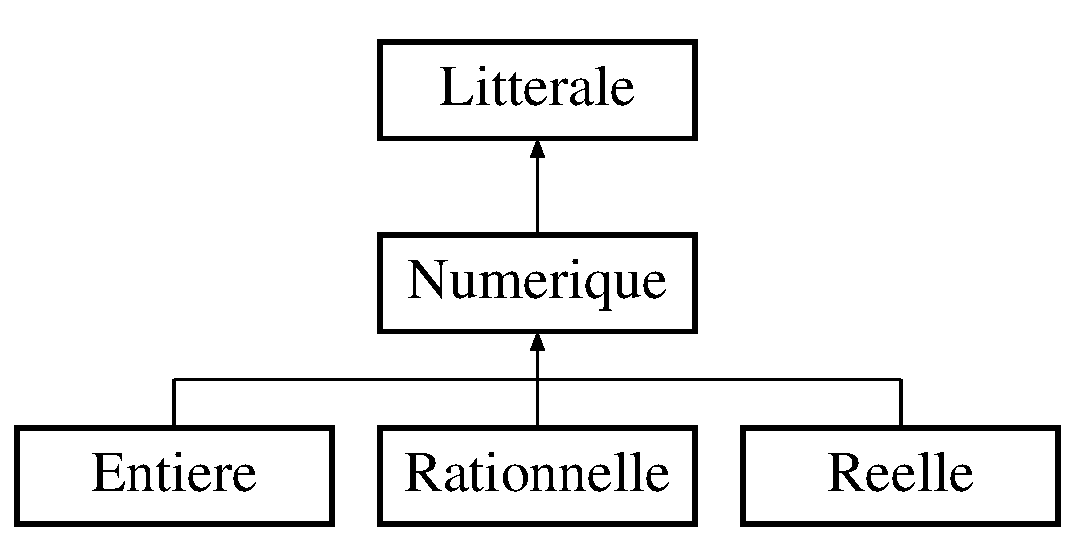
\includegraphics[height=3cm]{class_numerique}
\end{center}
\end{figure}
\subsection*{Fonctions membres publiques}
\begin{CompactItemize}
\item 
\hypertarget{class_numerique_f6d64b345f536d45454ba424d59a8ee4}{
virtual void \hyperlink{class_numerique_f6d64b345f536d45454ba424d59a8ee4}{affiche} () const =0}
\label{class_numerique_f6d64b345f536d45454ba424d59a8ee4}

\begin{CompactList}\small\item\em Redefinition de la fonction d'affichage. \item\end{CompactList}\item 
\hypertarget{class_numerique_5d88a526f166b01e5c116d7342daa7e8}{
virtual void \hyperlink{class_numerique_5d88a526f166b01e5c116d7342daa7e8}{neg} ()=0}
\label{class_numerique_5d88a526f166b01e5c116d7342daa7e8}

\begin{CompactList}\small\item\em Methode virtuelle pure permettant l'inversion du signe de la litterale. \item\end{CompactList}\item 
\hypertarget{class_numerique_facd4108df61baa46c639c8e15b23c7f}{
virtual \hyperlink{class_numerique}{Numerique} $\ast$ \hyperlink{class_numerique_facd4108df61baa46c639c8e15b23c7f}{clone} ()=0}
\label{class_numerique_facd4108df61baa46c639c8e15b23c7f}

\begin{CompactList}\small\item\em Redefinition de la fonction de clonage. \item\end{CompactList}\item 
\hypertarget{class_numerique_d6a208d078f63b62160d255a52c0ab1c}{
virtual double \hyperlink{class_numerique_d6a208d078f63b62160d255a52c0ab1c}{getComp} ()=0}
\label{class_numerique_d6a208d078f63b62160d255a52c0ab1c}

\begin{CompactList}\small\item\em Methode virtuelle pure permettant la recuperation de la valeur de la litterale sous forme de double pour comparaison. \item\end{CompactList}\end{CompactItemize}


\subsection{Description détaillée}
Classe abstraite representant un numerique, c'est a dire un nombre autre que complexe (heritage de \hyperlink{class_litterale}{Litterale}). 

La documentation de cette classe a été générée à partir du fichier suivant :\begin{CompactItemize}
\item 
Litterale.h\end{CompactItemize}

\hypertarget{class_pile}{
\section{Référence de la classe Pile}
\label{class_pile}\index{Pile@{Pile}}
}
Classe permettant de stocker les items sous forme de pile.  


{\tt \#include $<$Pile.h$>$}

\subsection*{Fonctions membres publiques}
\begin{CompactItemize}
\item 
\hypertarget{class_pile_b44e927107b28f5f3ac7697d10e0a739}{
\hyperlink{class_pile_b44e927107b28f5f3ac7697d10e0a739}{Pile} ()}
\label{class_pile_b44e927107b28f5f3ac7697d10e0a739}

\begin{CompactList}\small\item\em Constructeur. \item\end{CompactList}\item 
\hypertarget{class_pile_b2d1398d675586ff34994e2b109df152}{
\hyperlink{class_pile_b2d1398d675586ff34994e2b109df152}{$\sim$Pile} ()}
\label{class_pile_b2d1398d675586ff34994e2b109df152}

\begin{CompactList}\small\item\em Destructeur. \item\end{CompactList}\item 
\hypertarget{class_pile_874f209b5333810e6179b0061304b4e5}{
void \hyperlink{class_pile_874f209b5333810e6179b0061304b4e5}{affiche} () const }
\label{class_pile_874f209b5333810e6179b0061304b4e5}

\begin{CompactList}\small\item\em Affichage de la pile. \item\end{CompactList}\item 
void \hyperlink{class_pile_c61f214686f5c75fc71fc86ce8da53e0}{push} (\hyperlink{class_litterale}{Litterale} $\ast$const l)
\begin{CompactList}\small\item\em Insertion d'une litterale dans la pile. \item\end{CompactList}\item 
bool \hyperlink{class_pile_2ca7edab82a4b7a4305093dd9ab14d71}{estVide} () const 
\begin{CompactList}\small\item\em Test sur la capacite de la pile. \item\end{CompactList}\item 
int \hyperlink{class_pile_5d004688a405e8588c46336aa9cac0d9}{taille} () const 
\begin{CompactList}\small\item\em Accesseur sur le nombre. \item\end{CompactList}\item 
int \hyperlink{class_pile_b6c6dc3469f0ab644c5813f81f15b6dc}{tailleMax} () const 
\begin{CompactList}\small\item\em Accesseur sur le nombre maximum. \item\end{CompactList}\item 
\hyperlink{class_litterale}{Litterale} $\ast$const \hyperlink{class_pile_7e00e528aa0f5995a54941351659098f}{top} () const 
\begin{CompactList}\small\item\em Acces au dernier element. \item\end{CompactList}\item 
void \hyperlink{class_pile_a61a682bdd3b9dac5d1b25e481c453d1}{setNbItemsToAffiche} (unsigned int n)
\begin{CompactList}\small\item\em Accesseur sur le nombre a afficher. \item\end{CompactList}\item 
\hypertarget{class_pile_7488ed257c6ceb16ed57a9fffb0726d5}{
void \hyperlink{class_pile_7488ed257c6ceb16ed57a9fffb0726d5}{drop} ()}
\label{class_pile_7488ed257c6ceb16ed57a9fffb0726d5}

\begin{CompactList}\small\item\em Suppression du dernier element. \item\end{CompactList}\item 
\hypertarget{class_pile_2c9967dc8f5dcb4372475dee52ed64c6}{
void \hyperlink{class_pile_2c9967dc8f5dcb4372475dee52ed64c6}{swap} ()}
\label{class_pile_2c9967dc8f5dcb4372475dee52ed64c6}

\begin{CompactList}\small\item\em Inversion des deux derniers elements. \item\end{CompactList}\item 
\hypertarget{class_pile_a3991438f190580607d7bbbd50ecc0c3}{
void \hyperlink{class_pile_a3991438f190580607d7bbbd50ecc0c3}{clear} ()}
\label{class_pile_a3991438f190580607d7bbbd50ecc0c3}

\begin{CompactList}\small\item\em Suppression de l'integralite des elements de la pile. \item\end{CompactList}\item 
void \hyperlink{class_pile_47db93b6d3c9d527e9c4c8afb1565e2b}{reconstruire} (\hyperlink{class_memento}{Memento} m)
\begin{CompactList}\small\item\em Reconstruction de la pile suite a un REDO. \item\end{CompactList}\end{CompactItemize}
\subsection*{Amis}
\begin{CompactItemize}
\item 
\hypertarget{class_pile_15ea7cda491e1c5873aeba1aad9d457a}{
class \hyperlink{class_pile_15ea7cda491e1c5873aeba1aad9d457a}{Memento}}
\label{class_pile_15ea7cda491e1c5873aeba1aad9d457a}

\end{CompactItemize}


\subsection{Description détaillée}
Classe permettant de stocker les items sous forme de pile. 

\subsection{Documentation des fonctions membres}
\hypertarget{class_pile_2ca7edab82a4b7a4305093dd9ab14d71}{
\index{Pile@{Pile}!estVide@{estVide}}
\index{estVide@{estVide}!Pile@{Pile}}
\subsubsection[{estVide}]{\setlength{\rightskip}{0pt plus 5cm}bool Pile::estVide () const}}
\label{class_pile_2ca7edab82a4b7a4305093dd9ab14d71}


Test sur la capacite de la pile. 

\begin{Desc}
\item[Renvoie:]'true' si la pile est vide, 'false' sinon \end{Desc}
\hypertarget{class_pile_c61f214686f5c75fc71fc86ce8da53e0}{
\index{Pile@{Pile}!push@{push}}
\index{push@{push}!Pile@{Pile}}
\subsubsection[{push}]{\setlength{\rightskip}{0pt plus 5cm}void Pile::push ({\bf Litterale} $\ast$const  {\em l})}}
\label{class_pile_c61f214686f5c75fc71fc86ce8da53e0}


Insertion d'une litterale dans la pile. 

\begin{Desc}
\item[Paramètres:]
\begin{description}
\item[{\em l}]: pointeur sur la litterale a inserer \end{description}
\end{Desc}
\hypertarget{class_pile_47db93b6d3c9d527e9c4c8afb1565e2b}{
\index{Pile@{Pile}!reconstruire@{reconstruire}}
\index{reconstruire@{reconstruire}!Pile@{Pile}}
\subsubsection[{reconstruire}]{\setlength{\rightskip}{0pt plus 5cm}void Pile::reconstruire ({\bf Memento} {\em m})\hspace{0.3cm}{\tt  \mbox{[}inline\mbox{]}}}}
\label{class_pile_47db93b6d3c9d527e9c4c8afb1565e2b}


Reconstruction de la pile suite a un REDO. 

\begin{Desc}
\item[Paramètres:]
\begin{description}
\item[{\em m}]: memento du LitteralManager \end{description}
\end{Desc}
\hypertarget{class_pile_a61a682bdd3b9dac5d1b25e481c453d1}{
\index{Pile@{Pile}!setNbItemsToAffiche@{setNbItemsToAffiche}}
\index{setNbItemsToAffiche@{setNbItemsToAffiche}!Pile@{Pile}}
\subsubsection[{setNbItemsToAffiche}]{\setlength{\rightskip}{0pt plus 5cm}void Pile::setNbItemsToAffiche (unsigned int {\em n})}}
\label{class_pile_a61a682bdd3b9dac5d1b25e481c453d1}


Accesseur sur le nombre a afficher. 

\begin{Desc}
\item[Renvoie:]nombre d'items a afficher \end{Desc}
\hypertarget{class_pile_5d004688a405e8588c46336aa9cac0d9}{
\index{Pile@{Pile}!taille@{taille}}
\index{taille@{taille}!Pile@{Pile}}
\subsubsection[{taille}]{\setlength{\rightskip}{0pt plus 5cm}int Pile::taille () const}}
\label{class_pile_5d004688a405e8588c46336aa9cac0d9}


Accesseur sur le nombre. 

\begin{Desc}
\item[Renvoie:]nombre actuel d'items dans la pile \end{Desc}
\hypertarget{class_pile_b6c6dc3469f0ab644c5813f81f15b6dc}{
\index{Pile@{Pile}!tailleMax@{tailleMax}}
\index{tailleMax@{tailleMax}!Pile@{Pile}}
\subsubsection[{tailleMax}]{\setlength{\rightskip}{0pt plus 5cm}int Pile::tailleMax () const}}
\label{class_pile_b6c6dc3469f0ab644c5813f81f15b6dc}


Accesseur sur le nombre maximum. 

\begin{Desc}
\item[Renvoie:]nombre maximum d'items dans la pile \end{Desc}
\hypertarget{class_pile_7e00e528aa0f5995a54941351659098f}{
\index{Pile@{Pile}!top@{top}}
\index{top@{top}!Pile@{Pile}}
\subsubsection[{top}]{\setlength{\rightskip}{0pt plus 5cm}{\bf Litterale} $\ast$const Pile::top () const}}
\label{class_pile_7e00e528aa0f5995a54941351659098f}


Acces au dernier element. 

\begin{Desc}
\item[Renvoie:]pointeur sur la litterale au sommet de la pile \end{Desc}


La documentation de cette classe a été générée à partir des fichiers suivants :\begin{CompactItemize}
\item 
Pile.h\item 
Pile.cpp\end{CompactItemize}

\hypertarget{class_programme}{
\section{Référence de la classe Programme}
\label{class_programme}\index{Programme@{Programme}}
}
Classe representant un programme, c'est a dire une suite d'instructions (heritage de \hyperlink{class_litterale}{Litterale}).  


{\tt \#include $<$Litterale.h$>$}

Graphe d'héritage de Programme::\begin{figure}[H]
\begin{center}
\leavevmode
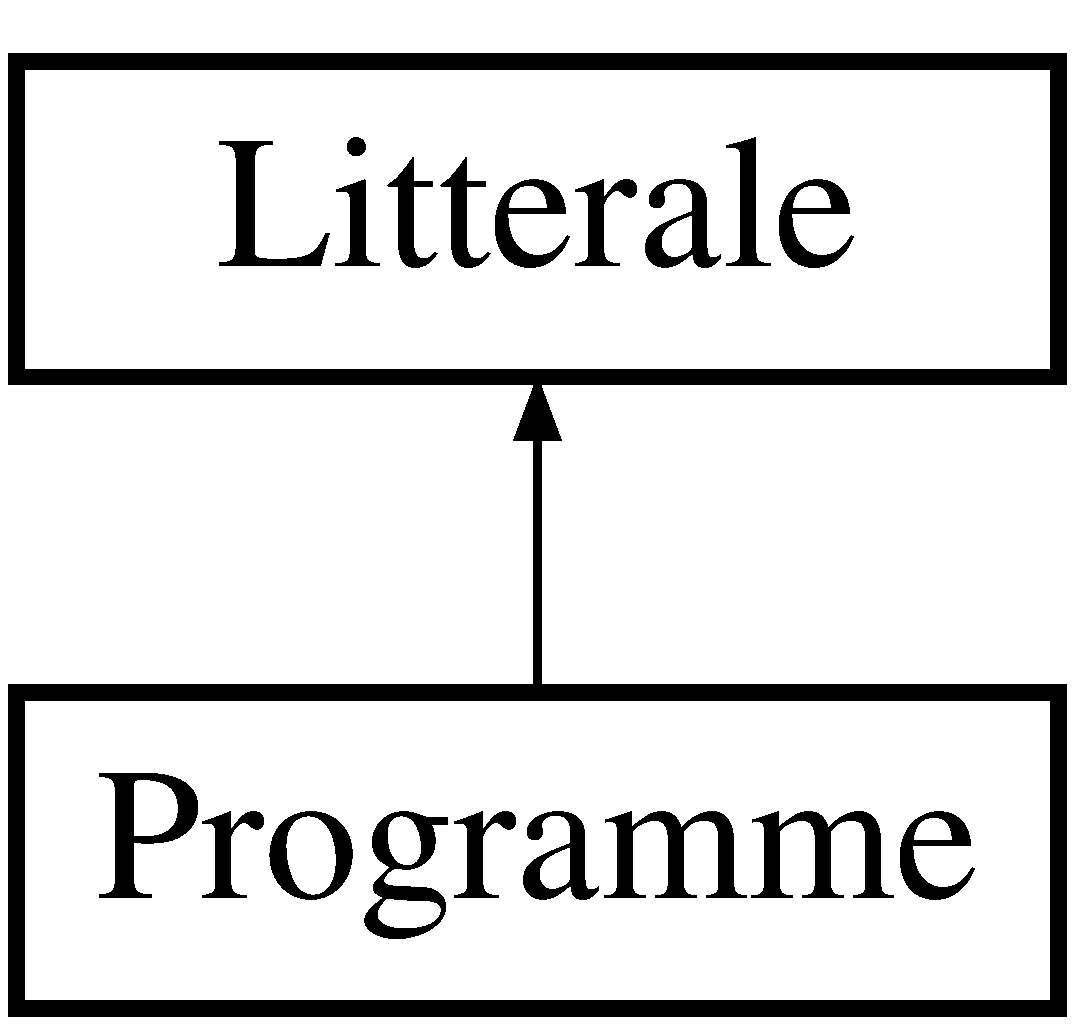
\includegraphics[height=2cm]{class_programme}
\end{center}
\end{figure}
\subsection*{Fonctions membres publiques}
\begin{CompactItemize}
\item 
\hyperlink{class_programme_714382be5455a92d17099406517df95f}{Programme} (string s)
\begin{CompactList}\small\item\em Constructeur. \item\end{CompactList}\item 
\hypertarget{class_programme_8a4a4047620cf9bf7b6682e4a8c0b850}{
void \hyperlink{class_programme_8a4a4047620cf9bf7b6682e4a8c0b850}{affiche} () const }
\label{class_programme_8a4a4047620cf9bf7b6682e4a8c0b850}

\begin{CompactList}\small\item\em Redefinition de la fonction d'affichage. \item\end{CompactList}\item 
string \hyperlink{class_programme_640770a1987a79ee81c985966254a959}{getProg} ()
\begin{CompactList}\small\item\em Accesseur. \item\end{CompactList}\item 
void \hyperlink{class_programme_db3fc4dc8b2751b3775a53fa245606d2}{edit} (string s)
\begin{CompactList}\small\item\em Editeur : permet de modifier le contenu du programme. \item\end{CompactList}\item 
\hypertarget{class_programme_df42f9872a754beefe020294f585f9a6}{
\hyperlink{class_programme}{Programme} $\ast$ \hyperlink{class_programme_df42f9872a754beefe020294f585f9a6}{clone} ()}
\label{class_programme_df42f9872a754beefe020294f585f9a6}

\begin{CompactList}\small\item\em Redefinition de la fonction de clonage. \item\end{CompactList}\end{CompactItemize}


\subsection{Description détaillée}
Classe representant un programme, c'est a dire une suite d'instructions (heritage de \hyperlink{class_litterale}{Litterale}). 

\subsection{Documentation des constructeurs et destructeur}
\hypertarget{class_programme_714382be5455a92d17099406517df95f}{
\index{Programme@{Programme}!Programme@{Programme}}
\index{Programme@{Programme}!Programme@{Programme}}
\subsubsection[{Programme}]{\setlength{\rightskip}{0pt plus 5cm}Programme::Programme (string {\em s})\hspace{0.3cm}{\tt  \mbox{[}inline\mbox{]}}}}
\label{class_programme_714382be5455a92d17099406517df95f}


Constructeur. 

\begin{Desc}
\item[Paramètres:]
\begin{description}
\item[{\em s}]: chaine de caractere representant le contenu du programme \end{description}
\end{Desc}


\subsection{Documentation des fonctions membres}
\hypertarget{class_programme_db3fc4dc8b2751b3775a53fa245606d2}{
\index{Programme@{Programme}!edit@{edit}}
\index{edit@{edit}!Programme@{Programme}}
\subsubsection[{edit}]{\setlength{\rightskip}{0pt plus 5cm}void Programme::edit (string {\em s})\hspace{0.3cm}{\tt  \mbox{[}inline\mbox{]}}}}
\label{class_programme_db3fc4dc8b2751b3775a53fa245606d2}


Editeur : permet de modifier le contenu du programme. 

\begin{Desc}
\item[Paramètres:]
\begin{description}
\item[{\em s}]: chaine de caracteres representant le nouveau contenu du programme \end{description}
\end{Desc}
\hypertarget{class_programme_640770a1987a79ee81c985966254a959}{
\index{Programme@{Programme}!getProg@{getProg}}
\index{getProg@{getProg}!Programme@{Programme}}
\subsubsection[{getProg}]{\setlength{\rightskip}{0pt plus 5cm}string Programme::getProg ()\hspace{0.3cm}{\tt  \mbox{[}inline\mbox{]}}}}
\label{class_programme_640770a1987a79ee81c985966254a959}


Accesseur. 

\begin{Desc}
\item[Renvoie:]chaine de caracteres representant le contenu du programme \end{Desc}


La documentation de cette classe a été générée à partir du fichier suivant :\begin{CompactItemize}
\item 
Litterale.h\end{CompactItemize}

\hypertarget{class_rationnelle}{
\section{Référence de la classe Rationnelle}
\label{class_rationnelle}\index{Rationnelle@{Rationnelle}}
}
Classe representant un nombre rationnel (heritage de \hyperlink{class_numerique}{Numerique}).  


{\tt \#include $<$Litterale.h$>$}

Graphe d'héritage de Rationnelle::\begin{figure}[H]
\begin{center}
\leavevmode
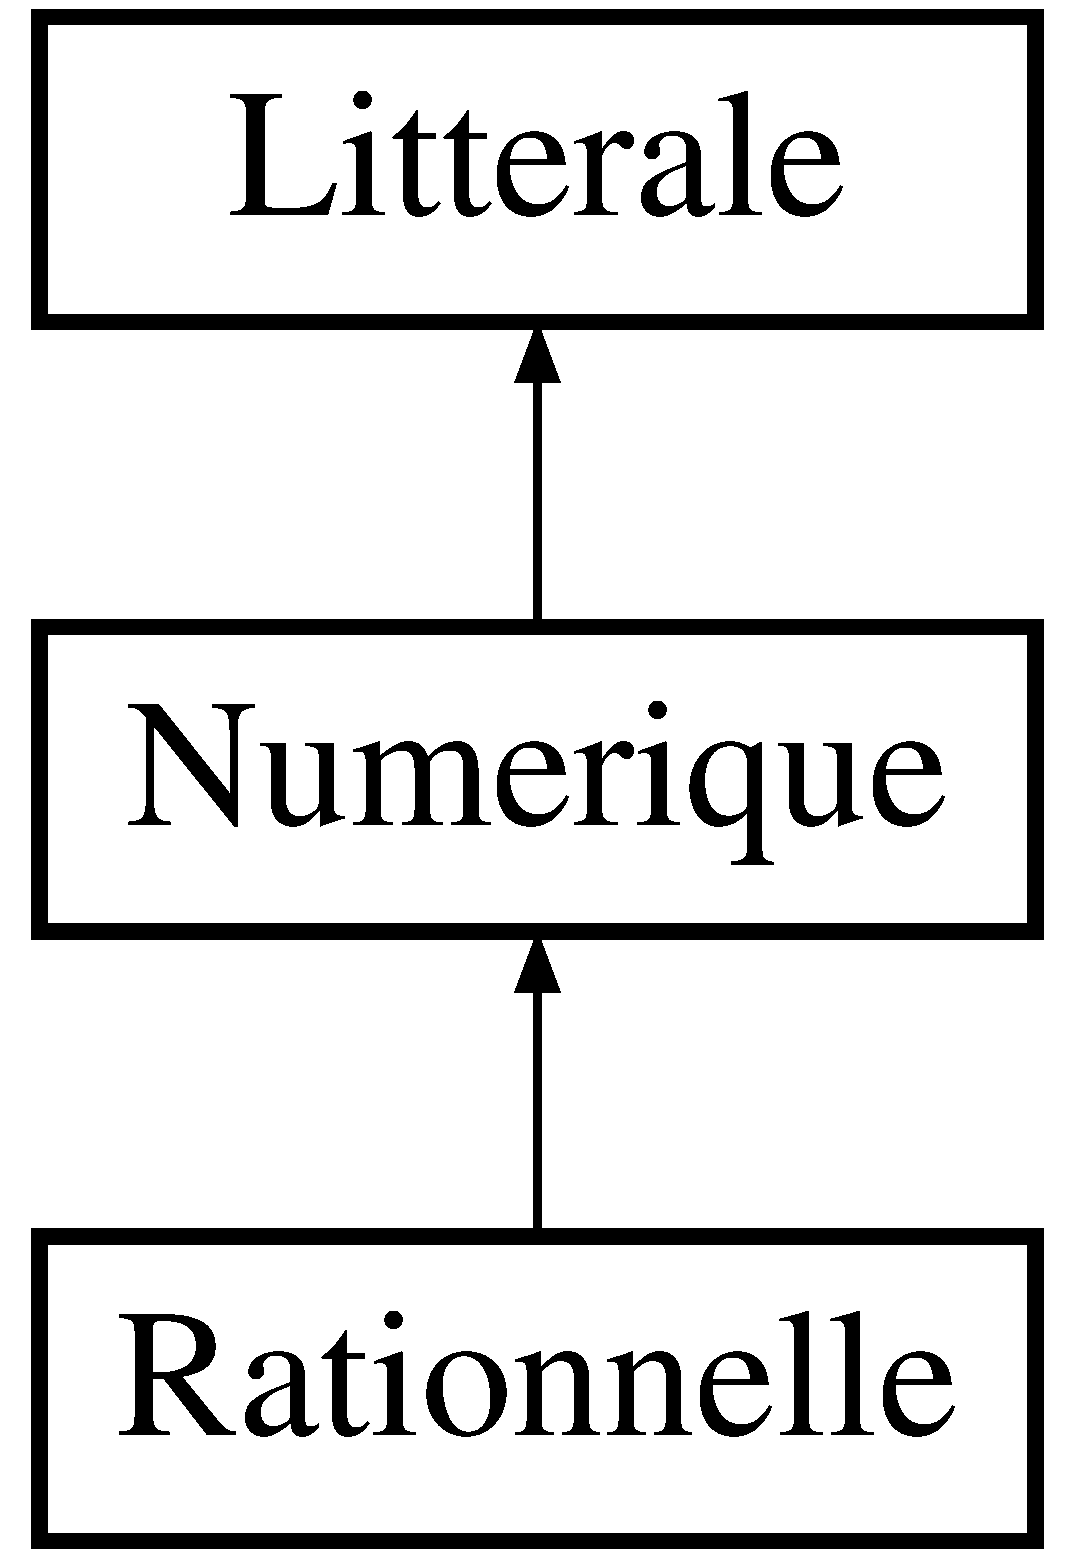
\includegraphics[height=3cm]{class_rationnelle}
\end{center}
\end{figure}
\subsection*{Fonctions membres publiques}
\begin{CompactItemize}
\item 
\hyperlink{class_rationnelle_80e2778456d58509340e31e304d77b8f}{Rationnelle} (\hyperlink{class_entiere}{Entiere} e1, \hyperlink{class_entiere}{Entiere} e2)
\begin{CompactList}\small\item\em Constructeur. \item\end{CompactList}\item 
\hypertarget{class_rationnelle_a4f581d2864da2bc7437a00b911377d9}{
void \hyperlink{class_rationnelle_a4f581d2864da2bc7437a00b911377d9}{simplification} ()}
\label{class_rationnelle_a4f581d2864da2bc7437a00b911377d9}

\begin{CompactList}\small\item\em Simplificateur de la fraction. \item\end{CompactList}\item 
\hyperlink{class_entiere}{Entiere} \hyperlink{class_rationnelle_a912b36ff009510986a131cf0d9d5c7b}{toEntiere} ()
\begin{CompactList}\small\item\em Construction d'une litterale entiere a partir d'une litterale rationnelle. \item\end{CompactList}\item 
\hyperlink{class_reelle}{Reelle} \hyperlink{class_rationnelle_ae003cf8f8f8fd3f8ca25833019293c7}{toReelle} ()
\begin{CompactList}\small\item\em Construction d'une litterale reelle a partir d'une litterale rationnelle. \item\end{CompactList}\item 
\hyperlink{class_entiere}{Entiere} \hyperlink{class_rationnelle_7bb78e18fcebedf67e29da7b8da56483}{getNum} () const 
\begin{CompactList}\small\item\em Accesseur sur le numerateur. \item\end{CompactList}\item 
\hyperlink{class_entiere}{Entiere} \hyperlink{class_rationnelle_fa5d908b5e2e972af5a431efb6686b52}{getDen} () const 
\begin{CompactList}\small\item\em Accesseur sur le denominateur. \item\end{CompactList}\item 
\hypertarget{class_rationnelle_7d5f7cf77d2c916b97f3697a071300df}{
void \hyperlink{class_rationnelle_7d5f7cf77d2c916b97f3697a071300df}{affiche} () const }
\label{class_rationnelle_7d5f7cf77d2c916b97f3697a071300df}

\begin{CompactList}\small\item\em Redefinition de la fonction d'affichage. \item\end{CompactList}\item 
\hypertarget{class_rationnelle_ba6dca31aee851018c69ac3c5b8dd81a}{
\hyperlink{class_rationnelle}{Rationnelle} $\ast$ \hyperlink{class_rationnelle_ba6dca31aee851018c69ac3c5b8dd81a}{clone} ()}
\label{class_rationnelle_ba6dca31aee851018c69ac3c5b8dd81a}

\begin{CompactList}\small\item\em Redefinition de la fonction de clonage. \item\end{CompactList}\item 
\hypertarget{class_rationnelle_1bb63e8e86011146a11507c948ed1410}{
void \hyperlink{class_rationnelle_1bb63e8e86011146a11507c948ed1410}{neg} ()}
\label{class_rationnelle_1bb63e8e86011146a11507c948ed1410}

\begin{CompactList}\small\item\em Redefinition de la fonction d'inversion de signe. \item\end{CompactList}\item 
\hypertarget{class_rationnelle_618f3d0c3b9bdb27bf279b8ecbb5a392}{
double \hyperlink{class_rationnelle_618f3d0c3b9bdb27bf279b8ecbb5a392}{getComp} ()}
\label{class_rationnelle_618f3d0c3b9bdb27bf279b8ecbb5a392}

\begin{CompactList}\small\item\em Redefinition de la fonction de clonage. \item\end{CompactList}\end{CompactItemize}


\subsection{Description détaillée}
Classe representant un nombre rationnel (heritage de \hyperlink{class_numerique}{Numerique}). 

\subsection{Documentation des constructeurs et destructeur}
\hypertarget{class_rationnelle_80e2778456d58509340e31e304d77b8f}{
\index{Rationnelle@{Rationnelle}!Rationnelle@{Rationnelle}}
\index{Rationnelle@{Rationnelle}!Rationnelle@{Rationnelle}}
\subsubsection[{Rationnelle}]{\setlength{\rightskip}{0pt plus 5cm}Rationnelle::Rationnelle ({\bf Entiere} {\em e1}, \/  {\bf Entiere} {\em e2})\hspace{0.3cm}{\tt  \mbox{[}inline\mbox{]}}}}
\label{class_rationnelle_80e2778456d58509340e31e304d77b8f}


Constructeur. 

\begin{Desc}
\item[Paramètres:]
\begin{description}
\item[{\em e1}]: entiere representant le numerateur \item[{\em e2}]: entiere representant le denominateur \end{description}
\end{Desc}


\subsection{Documentation des fonctions membres}
\hypertarget{class_rationnelle_fa5d908b5e2e972af5a431efb6686b52}{
\index{Rationnelle@{Rationnelle}!getDen@{getDen}}
\index{getDen@{getDen}!Rationnelle@{Rationnelle}}
\subsubsection[{getDen}]{\setlength{\rightskip}{0pt plus 5cm}{\bf Entiere} Rationnelle::getDen () const\hspace{0.3cm}{\tt  \mbox{[}inline\mbox{]}}}}
\label{class_rationnelle_fa5d908b5e2e972af5a431efb6686b52}


Accesseur sur le denominateur. 

\begin{Desc}
\item[Renvoie:]valeur du denominateur de la fraction (litterale entiere) \end{Desc}
\hypertarget{class_rationnelle_7bb78e18fcebedf67e29da7b8da56483}{
\index{Rationnelle@{Rationnelle}!getNum@{getNum}}
\index{getNum@{getNum}!Rationnelle@{Rationnelle}}
\subsubsection[{getNum}]{\setlength{\rightskip}{0pt plus 5cm}{\bf Entiere} Rationnelle::getNum () const\hspace{0.3cm}{\tt  \mbox{[}inline\mbox{]}}}}
\label{class_rationnelle_7bb78e18fcebedf67e29da7b8da56483}


Accesseur sur le numerateur. 

\begin{Desc}
\item[Renvoie:]valeur du numerateur de la fraction (litterale entiere) \end{Desc}
\hypertarget{class_rationnelle_a912b36ff009510986a131cf0d9d5c7b}{
\index{Rationnelle@{Rationnelle}!toEntiere@{toEntiere}}
\index{toEntiere@{toEntiere}!Rationnelle@{Rationnelle}}
\subsubsection[{toEntiere}]{\setlength{\rightskip}{0pt plus 5cm}{\bf Entiere} Rationnelle::toEntiere ()\hspace{0.3cm}{\tt  \mbox{[}inline\mbox{]}}}}
\label{class_rationnelle_a912b36ff009510986a131cf0d9d5c7b}


Construction d'une litterale entiere a partir d'une litterale rationnelle. 

\begin{Desc}
\item[Renvoie:]litterale entiere \end{Desc}
\hypertarget{class_rationnelle_ae003cf8f8f8fd3f8ca25833019293c7}{
\index{Rationnelle@{Rationnelle}!toReelle@{toReelle}}
\index{toReelle@{toReelle}!Rationnelle@{Rationnelle}}
\subsubsection[{toReelle}]{\setlength{\rightskip}{0pt plus 5cm}{\bf Reelle} Rationnelle::toReelle ()\hspace{0.3cm}{\tt  \mbox{[}inline\mbox{]}}}}
\label{class_rationnelle_ae003cf8f8f8fd3f8ca25833019293c7}


Construction d'une litterale reelle a partir d'une litterale rationnelle. 

\begin{Desc}
\item[Renvoie:]litterale reelle \end{Desc}


La documentation de cette classe a été générée à partir des fichiers suivants :\begin{CompactItemize}
\item 
Litterale.h\item 
Litterale.cpp\end{CompactItemize}

\hypertarget{class_reelle}{
\section{Référence de la classe Reelle}
\label{class_reelle}\index{Reelle@{Reelle}}
}
Classe representant un nombre reel (heritage de \hyperlink{class_numerique}{Numerique}).  


{\tt \#include $<$Litterale.h$>$}

Graphe d'héritage de Reelle::\begin{figure}[H]
\begin{center}
\leavevmode
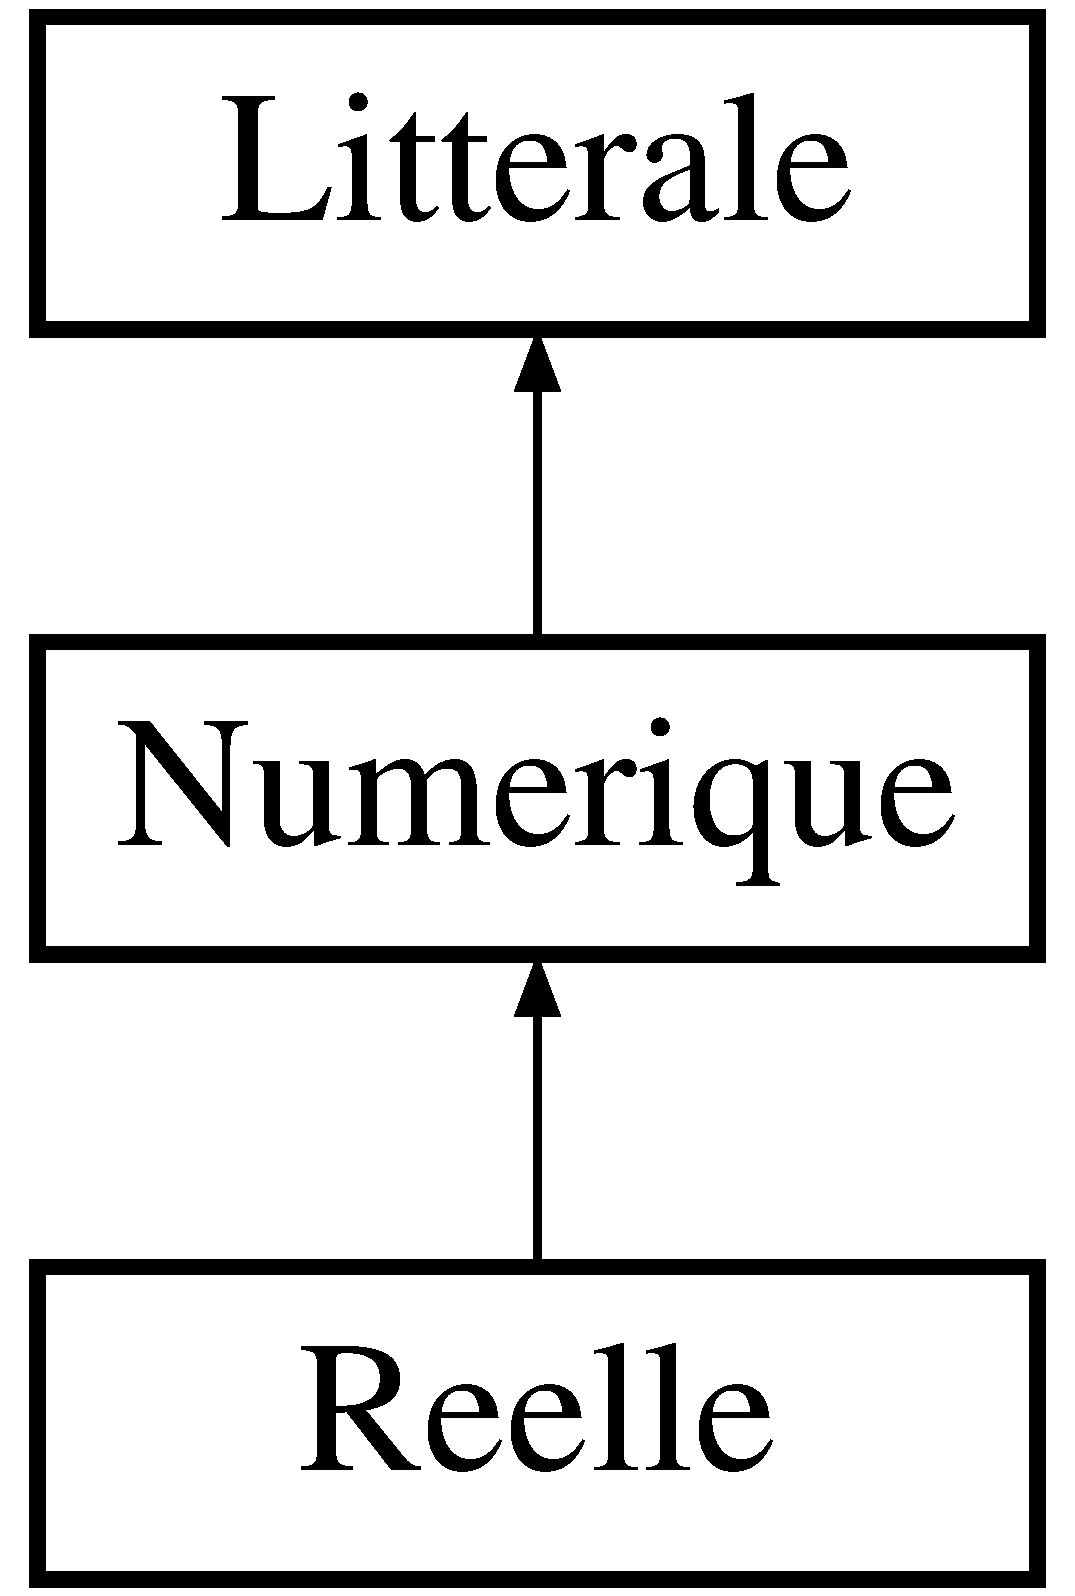
\includegraphics[height=3cm]{class_reelle}
\end{center}
\end{figure}
\subsection*{Fonctions membres publiques}
\begin{CompactItemize}
\item 
\hyperlink{class_reelle_6fdee6f1628064efbfe4bdcd31a8cfc4}{Reelle} (double v)
\begin{CompactList}\small\item\em Constructeur. \item\end{CompactList}\item 
\hyperlink{class_entiere}{Entiere} \hyperlink{class_reelle_9a9cb01d74565fa4e702044ffc3fceb7}{toEntiere} ()
\begin{CompactList}\small\item\em Construction d'une litterale \hyperlink{class_entiere}{Entiere} a partir d'une litterale reelle. \item\end{CompactList}\item 
double \hyperlink{class_reelle_5ebbb4a65a1143c736b8545fc67af281}{getVal} () const 
\begin{CompactList}\small\item\em Accesseur. \item\end{CompactList}\item 
\hypertarget{class_reelle_df93b60f8c72687b412e7589a2be114c}{
void \hyperlink{class_reelle_df93b60f8c72687b412e7589a2be114c}{affiche} () const }
\label{class_reelle_df93b60f8c72687b412e7589a2be114c}

\begin{CompactList}\small\item\em Redefinition de la fonction d'affichage. \item\end{CompactList}\item 
\hypertarget{class_reelle_3141e2961030350942c10de764c13180}{
\hyperlink{class_reelle}{Reelle} $\ast$ \hyperlink{class_reelle_3141e2961030350942c10de764c13180}{clone} ()}
\label{class_reelle_3141e2961030350942c10de764c13180}

\begin{CompactList}\small\item\em Redefinition de la fonction de clonage. \item\end{CompactList}\item 
\hypertarget{class_reelle_a3b7da9b29f96a45b2064f7918d014c3}{
void \hyperlink{class_reelle_a3b7da9b29f96a45b2064f7918d014c3}{neg} ()}
\label{class_reelle_a3b7da9b29f96a45b2064f7918d014c3}

\begin{CompactList}\small\item\em Redefinition de la fonction d'inversion de signe. \item\end{CompactList}\item 
\hypertarget{class_reelle_5a32997cd26bb14a9445e06b0bd94f29}{
double \hyperlink{class_reelle_5a32997cd26bb14a9445e06b0bd94f29}{getComp} ()}
\label{class_reelle_5a32997cd26bb14a9445e06b0bd94f29}

\begin{CompactList}\small\item\em Redefinition de la fonction de comparaison. \item\end{CompactList}\end{CompactItemize}


\subsection{Description détaillée}
Classe representant un nombre reel (heritage de \hyperlink{class_numerique}{Numerique}). 

\subsection{Documentation des constructeurs et destructeur}
\hypertarget{class_reelle_6fdee6f1628064efbfe4bdcd31a8cfc4}{
\index{Reelle@{Reelle}!Reelle@{Reelle}}
\index{Reelle@{Reelle}!Reelle@{Reelle}}
\subsubsection[{Reelle}]{\setlength{\rightskip}{0pt plus 5cm}Reelle::Reelle (double {\em v})\hspace{0.3cm}{\tt  \mbox{[}inline\mbox{]}}}}
\label{class_reelle_6fdee6f1628064efbfe4bdcd31a8cfc4}


Constructeur. 

\begin{Desc}
\item[Paramètres:]
\begin{description}
\item[{\em v}]: valeur de la litterale \hyperlink{class_reelle}{Reelle} \end{description}
\end{Desc}


\subsection{Documentation des fonctions membres}
\hypertarget{class_reelle_5ebbb4a65a1143c736b8545fc67af281}{
\index{Reelle@{Reelle}!getVal@{getVal}}
\index{getVal@{getVal}!Reelle@{Reelle}}
\subsubsection[{getVal}]{\setlength{\rightskip}{0pt plus 5cm}double Reelle::getVal () const\hspace{0.3cm}{\tt  \mbox{[}inline\mbox{]}}}}
\label{class_reelle_5ebbb4a65a1143c736b8545fc67af281}


Accesseur. 

\begin{Desc}
\item[Renvoie:]v : valeur de la litterale \hyperlink{class_reelle}{Reelle} \end{Desc}
\hypertarget{class_reelle_9a9cb01d74565fa4e702044ffc3fceb7}{
\index{Reelle@{Reelle}!toEntiere@{toEntiere}}
\index{toEntiere@{toEntiere}!Reelle@{Reelle}}
\subsubsection[{toEntiere}]{\setlength{\rightskip}{0pt plus 5cm}{\bf Entiere} Reelle::toEntiere ()\hspace{0.3cm}{\tt  \mbox{[}inline\mbox{]}}}}
\label{class_reelle_9a9cb01d74565fa4e702044ffc3fceb7}


Construction d'une litterale \hyperlink{class_entiere}{Entiere} a partir d'une litterale reelle. 

\begin{Desc}
\item[Renvoie:]litterale entiere \end{Desc}


La documentation de cette classe a été générée à partir du fichier suivant :\begin{CompactItemize}
\item 
Litterale.h\end{CompactItemize}

\chapter{Documentation des fichiers}
\hypertarget{_computer_exception_8h}{
\section{Référence du fichier ComputerException.h}
\label{_computer_exception_8h}\index{ComputerException.h@{ComputerException.h}}
}
Gestion des erreurs.  


{\tt \#include $<$string$>$}\par
\subsection*{Classes}
\begin{CompactItemize}
\item 
class \hyperlink{class_computer_exception}{ComputerException}
\begin{CompactList}\small\item\em Classe permettant la gestion des erreurs. \item\end{CompactList}\end{CompactItemize}


\subsection{Description détaillée}
Gestion des erreurs. 

\begin{Desc}
\item[Auteur:]Felix ALIE \& Clement ROUTIER \end{Desc}
\begin{Desc}
\item[Version:]1 \end{Desc}

\hypertarget{_controleur_8h}{
\section{Référence du fichier Controleur.h}
\label{_controleur_8h}\index{Controleur.h@{Controleur.h}}
}
Base de lancement de l'application.  


{\tt \#include \char`\"{}LitteraleManager.h\char`\"{}}\par
{\tt \#include \char`\"{}Litterale.h\char`\"{}}\par
{\tt \#include \char`\"{}Pile.h\char`\"{}}\par
{\tt \#include \char`\"{}ComputerException.h\char`\"{}}\par
{\tt \#include \char`\"{}HashMap.h\char`\"{}}\par
{\tt \#include $<$regex$>$}\par
{\tt \#include $<$string$>$}\par
{\tt \#include $<$iostream$>$}\par
{\tt \#include $<$sstream$>$}\par
\subsection*{Classes}
\begin{CompactItemize}
\item 
class \hyperlink{class_controleur}{Controleur}
\begin{CompactList}\small\item\em Classe permettant de gerer l'ensemble de la calculatrice. \item\end{CompactList}\end{CompactItemize}


\subsection{Description détaillée}
Base de lancement de l'application. 

Gestion de la pile et de ses items.

Gestion de l'ensemble des litterales.

Ensemble des classes litterales.

Table de stockage et variables et des programmes.

\begin{Desc}
\item[Auteur:]Felix ALIE \& Clement ROUTIER \end{Desc}
\begin{Desc}
\item[Version:]1 \end{Desc}

\printindex
\end{document}
